\documentclass{beamer}

\mode<presentation> {
	\usetheme{Boadilla}
	%\usetheme{CambridgeUS}
}
\usefonttheme[onlymath]{serif}
\usepackage{graphicx}
\usepackage{booktabs} % Allows the use of \toprule, \midrule and \bottomrule in tables
\usepackage{amsmath}
\usepackage{amsfonts}
\usepackage{enumerate}
\usepackage{color}
%-------------------------------------------------------------------------
\title[Q. J. Econ, 2013]{The Transitional Costs of Sectoral Reallocation \\ {\small Evidence from the Clean Air Act and the Workforce}}
\author{W. Reed Walker} 
\institute[]{Presenter: Qinzhu Sun}

\date{\today}
\logo{
\includegraphics[scale=0.2]{maingate2}}
\begin{document}

\begin{frame}
	\titlepage
\end{frame}

\begin{frame}{Overview}
	\tableofcontents
\end{frame}
%-------------------------------------------------------------------------
%-------------------------------------------------------------------------
\section{Introduction}
\begin{frame}[shrink]
	\transfade %fade in and fade out
	\tableofcontents[sectionstyle=show/shaded,subsectionstyle=show/shaded/hide]
	\addtocounter{framenumber}{-1}
\end{frame}
%------------------------------------------------
\begin{frame}{Motivation}
	Environmental policies have large health benefits, while they also come with costs. Production is typically reallocated away from newly regulated industries to other sectors and locations.
	\medskip

	\textbf{Two possibilities concerning labor input reallocation (jobs lost):}
	\begin{itemize}
		\item Workers simply transition from one employer to the next without significant earnings loss.
		\item Workers lose job- or industry-specific skills and/or experience long periods of unemployment following job transitions. There also may be costs to workers who remain in these potentially less productive industries.
	\end{itemize}
	$\Rightarrow$ which is true?
\end{frame}
%------------------------------------------------
\begin{frame}{Literature Review}
	The analysis relates to a large literature on the costs and incidence of labor market adjustment to external factors, such as trade, immigration, or innovations in labor demand.
	\medskip

	\begin{itemize}
		\item Traditionally, work in this area examines how prices in industries or regional labor markets respond to external labor market shocks, and then the estimates are used to back out a measure of welfare or incidence.
		\item In contrast, this study is able to observe and estimate both worker-specific nonemployment durations and any long-run earnings changes associated with the reallocation of production and workers.
	\end{itemize}
\end{frame}
%------------------------------------------------
\begin{frame}{Literature Review}
	This article departs from the existing literature in four important ways.
	\begin{enumerate}
		\item While interpreting the job loss effects coming with environmental regulations, seldom does prior research know about the \textcolor{red}{long-run earnings losses} associated with these job transitions.
		\item Industry-level wage and employment data are likely to be misleading in terms of labor market incidence. In contrast, I exploit detailed longitudinal data to \textcolor{red}{follow workers over time and across jobs}.
		\item This paper uses a new, plant-level dataset from EPA that details exactly which plants are regulated under the various environmental programs in US. I match this database to administrative, plant-level data from the U.S. Census Bureau, \textcolor{red}{allowing me to observe plant-level regulatory status over time}.
		\item This article also lends insight as to how workers and labor markets adjust to sector specific shocks.
	\end{enumerate}
\end{frame}
%------------------------------------------------
\begin{frame}{Main Findings}
	\begin{itemize}
		\item The reallocative costs to the workforce from the 1990 CAAA are significant.
		\item For those workers in the regulated sector prior to the change in regulation, the average earnings declined by more than 5\% in the three years after theregulation.
		\item Almost all of the estimated earnings losses are driven by workers who separate from their firm.
		\item There is also substantial cross-sectional heterogeneity in the regulatory impact.
	\end{itemize}
\end{frame}
%-------------------------------------------------------------------------
%-------------------------------------------------------------------------
\section{The Clean Air Act and Environmental Regulation}
\begin{frame}[shrink]
	\transfade %fade in and fade out
	\tableofcontents[sectionstyle=show/shaded,subsectionstyle=show/shaded/hide]
	\addtocounter{framenumber}{-1}
\end{frame}
%------------------------------------------------
\begin{frame}{The Clean Air Act and Environmental Regulation}
	Air pollution regulation in the US is coordinated under the Clean Air Act(CAA), the largest environmental program in the nation.
	\begin{itemize}
		\item The act was passed in 1963 and amended in 1970, 1977, and 1990.
		\item The 1977 CAAA stipulated that every county in the US must be designated annually as being in attainment or out of attainment (nonattainment) of national ambient air quality standards (NAAQS).
		\begin{itemize}
			\item When a county is out of attainment for one of the regulated pollutants, the EPA requires states to adopt regulatory plans, known as state implementation plans(SIPs), to bring their county into compliance.
		\end{itemize}
		\item The CAAA of 1990 officially designated a set of counties as nonattainment for a new particulate matter standard (PM10) while also formally requiring all polluters of criteria air pollutants to obtain an operating permit.
	\end{itemize}
\end{frame}
%-------------------------------------------------------------------------
%-------------------------------------------------------------------------
\section{The Clean Air Act as a Research Design}
\begin{frame}[shrink]
	\transfade %fade in and fade out
	\tableofcontents[sectionstyle=show/shaded,subsectionstyle=show/shaded/hide]
	\addtocounter{framenumber}{-1}
\end{frame}
%------------------------------------------------
\begin{frame}{The Clean Air Act as a Research Design}
	A naive comparison of earnings in polluting and nonpolluting firms of nonattainment counties is likely to yield biased estimates.
	\begin{itemize}
		\item Wages vary tremendously across both firms and locations for reasons observed and unobserved to the econometrician.
		\item Moreover, this variation in the wage structure is likely correlated with a firm's status as a polluter.
		\item Workers may also demand some form of compensating wage differential associated with potentially harmful working conditions.
	\end{itemize}
	$\Rightarrow$ The CAA is a good natural experiment.
	\begin{itemize}
		\item It is possible to estimate models that include flexible controls for nationwide or industry-specific shocks to employment and/or earnings.
		\item Temporal variation in regulations exists from counties that go in and out of nonattainment based on annual pollution levels, allowing for pre/post comparisons within counties, industries, plants, or workers.
		\begin{itemize}
			\item Any time-invariant unobservables unique to these groups may be controlled for by including a set of group-specific fixed effects.
		\end{itemize}
	\end{itemize}
\end{frame}
%------------------------------------------------
\begin{frame}{The Clean Air Act as a Research Design}
	\textbf{Endogeneity:} A potential issue with time series variation in light of nonattainment designation is that pollution is correlated with economic activity (Chay and Greenstone, 2003b).

	$\Rightarrow$ This study relies on the discrete policy change of the 1990 CAAA.
	\begin{itemize}
		\item As mentioned, the 1990 CAAA were implemented in a way such that a handful of counties suddenly found themselves in nonattainment relative to the year prior.
	\end{itemize}
	\medskip

	\textbf{Last,} within any nonattainment county, only polluting plants are regulated, only if they emit the specific pollutant for which the county is in violation.
	\begin{itemize}
		\item Because only the polluting firms within a given county-industry are regulated, it is possible to control for unobservable, county-level (or county-by-industry level) changes in local economic conditions.
	\end{itemize}
\end{frame}
%------------------------------------------------
\begin{frame}{The Clean Air Act as a Research Design}
	\begin{figure}[h]
		\centering
		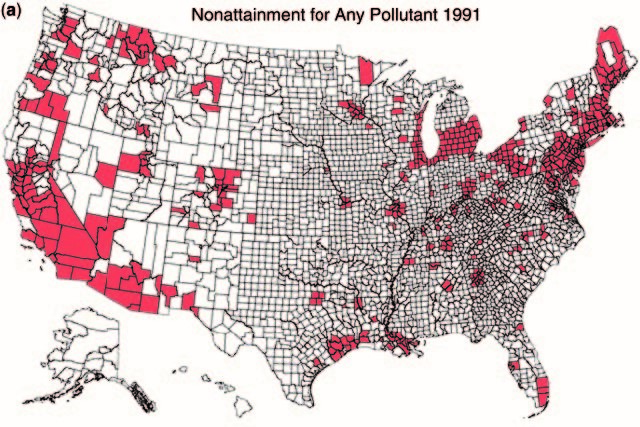
\includegraphics[scale=1.1]{figure1a.jpg}
	\end{figure}
\end{frame}
%------------------------------------------------
\begin{frame}{The Clean Air Act as a Research Design}
	\begin{figure}[h]
		\centering
		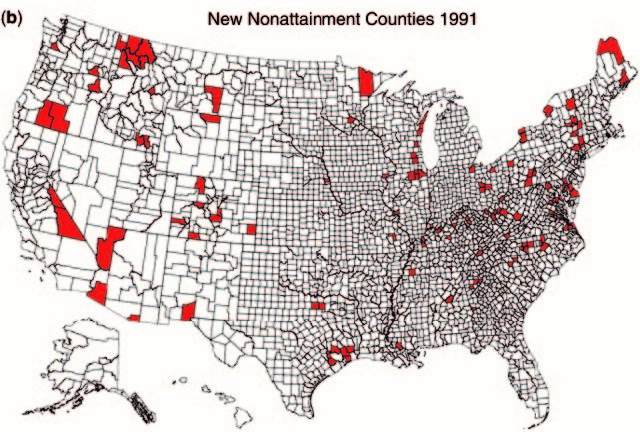
\includegraphics[scale=1.1]{figure1b.jpg}
	\end{figure}
\end{frame}
%------------------------------------------------
\begin{frame}{The Clean Air Act as a Research Design}{Summary}
	All of these sources of variation amount to a research design that \textcolor{red}{examines the earnings outcomes of workers in polluting plants of newly regulated counties, before and after the introduction of the plant-level regulations}.
	
	$\Rightarrow$ \textbf{DDD}
\end{frame}
%-------------------------------------------------------------------------
%-------------------------------------------------------------------------
\section{Data Overview and Description}
\begin{frame}[shrink]
	\transfade %fade in and fade out
	\tableofcontents[sectionstyle=show/shaded,subsectionstyle=show/shaded/hide]
	\addtocounter{framenumber}{-1}
\end{frame}
%------------------------------------------------
\begin{frame}{Data Overview and Description}
	\textbf{A. The Longitudinal Employer Household Dynamics Files}
	\begin{itemize}
		\item The Census Bureau’s LEHD file provides administrative, quarterly earnings records for a large percentage of the U.S. workforce.
		\item The LEHD also provides important demographic information on workers such as age, race, and education as well as time-varying information from the firms at which they work.
		\item Sample restrictions: only workers who worked in the manufacturing and electric/gas industries (i.e., two-digit SIC 20–39, 49) in 1990.
	\end{itemize}
	\textbf{B. Longitudinal Business Database}
	\begin{itemize}
		\item LBD is a plant-level database that covers the universe of establishments in the US from 1975 to 2005.
		\item Goal: assess the pre-CAAA trends, since the LEHD contains earnings records only as far back as 1990 (\& CAAA went into place in 1991).
		\item Observed are trends in employment and earnings per worker before and after these changes for newly affected sectors relative to unaffected sectors.
	\end{itemize}
\end{frame}
%------------------------------------------------
\begin{frame}{Data Overview and Description}
	\textbf{C. EPA Air Facility Subsystem}
	\begin{itemize}
		\item EPA AFS is a plant-level database that provides information detailing the regulatory programs for which the plant is permitted (and regulated) \& the specific pollutants for which the permit is issued.
		\item This project is the first to use the AFS data to examine the effects of plant-level regulatory status on firm and worker outcomes.
	\end{itemize}
	\textbf{D. Aggregation}
	\begin{itemize}
		\item First, I use the LBD to calculate mean earnings per worker and total employment in a county$\times$sector$\times$year, where a sector is based on the polluting status of a plant.
		\item The second form of aggregation uses the LEHD to calculate the mean "cohort" earnings by collapsing the micro-data to the cohort$\times$year.
	\end{itemize}
\end{frame}
%------------------------------------------------
\begin{frame}{Data Overview and Description}
	\textbf{E. Baseline Industry and Worker Characteristics}
	\begin{figure}[h]
		\centering
		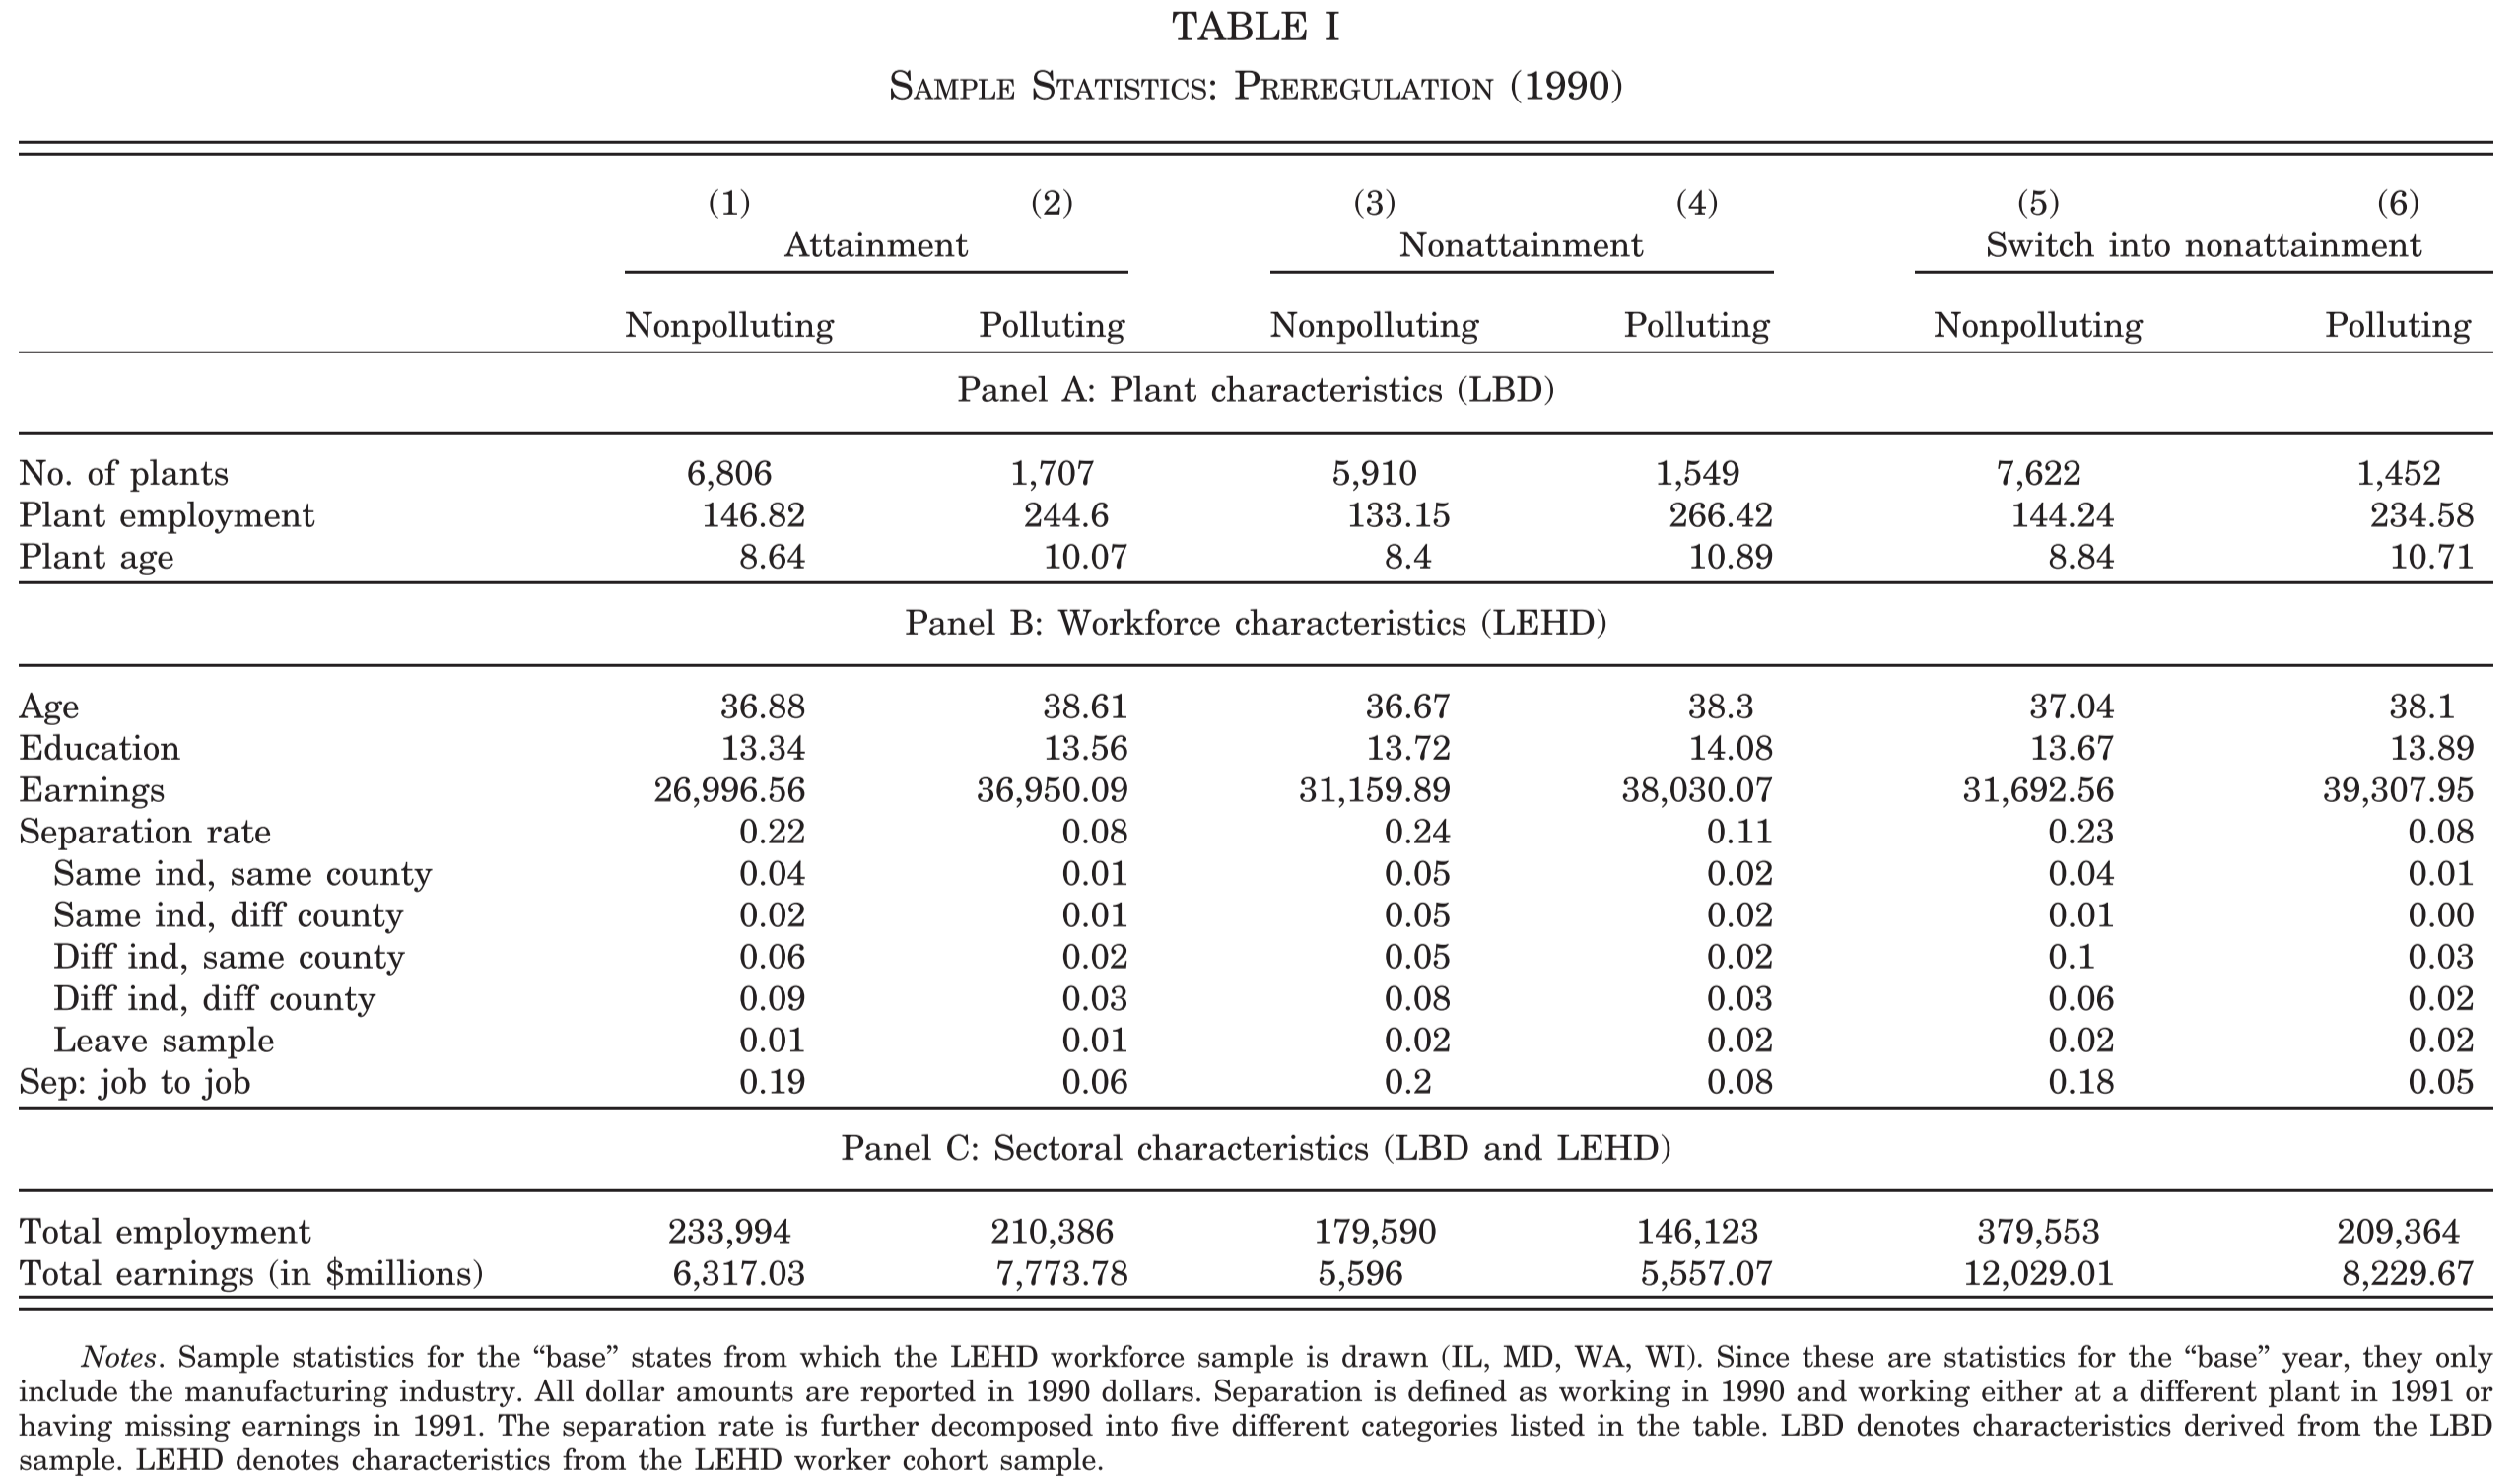
\includegraphics[scale=0.35]{table1.png}
	\end{figure}
\end{frame}
%-------------------------------------------------------------------------
%-------------------------------------------------------------------------
\section{Measurement Framework}
\begin{frame}[shrink]
	\transfade %fade in and fade out
	\tableofcontents[sectionstyle=show/shaded,subsectionstyle=show/shaded/hide]
	\addtocounter{framenumber}{-1}
\end{frame}
%------------------------------------------------
\begin{frame}{Measurement Framework}
	\begin{equation}
		Y_{jcst} = {\color{red}\eta_1}\left[N_c^\rho\times P_s^\rho\times 1(\tau_t>0)\right]+\chi_{jcs}+n_{ct}+p_{st}+\Phi_{jt}+\epsilon_{jcst}
	\end{equation}

	\textbf{Three margins of variation:}
	\begin{itemize}
		\item County nonattainment status\footnote{County nonattainment designations are pollutant-specific, and they apply only to plants that emit the regulated pollutant.}: $c\in \mbox{\{Attain, Nonattain\}}$
		\item Sectoral polluter status: $s\in 2^\Omega$, $ \Omega = \mbox{\{PM10, ozone\}}$
		\item Two time periods: $\tau\in\mbox{\{Pre, Post\}}$
	\end{itemize}
	\textbf{Denotation:}
	\begin{itemize}
		\item $Y_{jcst}$: outcome variable (i.e. earnings and employment);
		\item $N_c^\rho$: indicator equal to 1 for counties that were newly designated as nonattainment for pollutant $\rho$;
		\item $P_s^\rho$: indicator for the sector of plants that emit pollutant $\rho$;
		\item $1(\tau_t>0)$: indicator for the years after introducing new regulations.
	\end{itemize}
\end{frame}
%------------------------------------------------
\begin{frame}{Measurement Framework}
	\textbf{Event-study approach:}
	\begin{equation}
		Y_{jcst} = \sum_{k=-m}^M{\color{red}\eta_1^k}\left[N_c\times P_s\times 1(\tau_t=k)\right]+\chi_{jcs}+n_{ct}+p_{st}+\Phi_{jt}+\epsilon_{jcst}
	\end{equation}
	\begin{block}{Identifying assumption}
		No other factors generating a difference in differential trends between production decisions in regulated and unregulated manufacturing firms.
	\end{block}
	$\Rightarrow$ \textbf{Indirect tests:}
	\begin{itemize}
		\item Pre-trend;
		\item Check through the regulatory structure.
	\end{itemize}
\end{frame}
%-------------------------------------------------------------------------
%-------------------------------------------------------------------------
\section{Results}
\begin{frame}[shrink]
	\transfade %fade in and fade out
	\tableofcontents[sectionstyle=show/shaded,subsectionstyle=show/shaded/hide]
	\addtocounter{framenumber}{-1}
\end{frame}
%------------------------------------------------
\begin{frame}[label=figure2]{A.Regulation Leads to a Reduction in Sectoral Employment}
	Begin by estimating the degree to which \textcolor{red}{sectoral (not plant)}\footnote{reflect employment flows on both the intensive and extensive plant operating margin} employment responds to changes in environmental regulations.
	\begin{figure}[h]
		\centering
		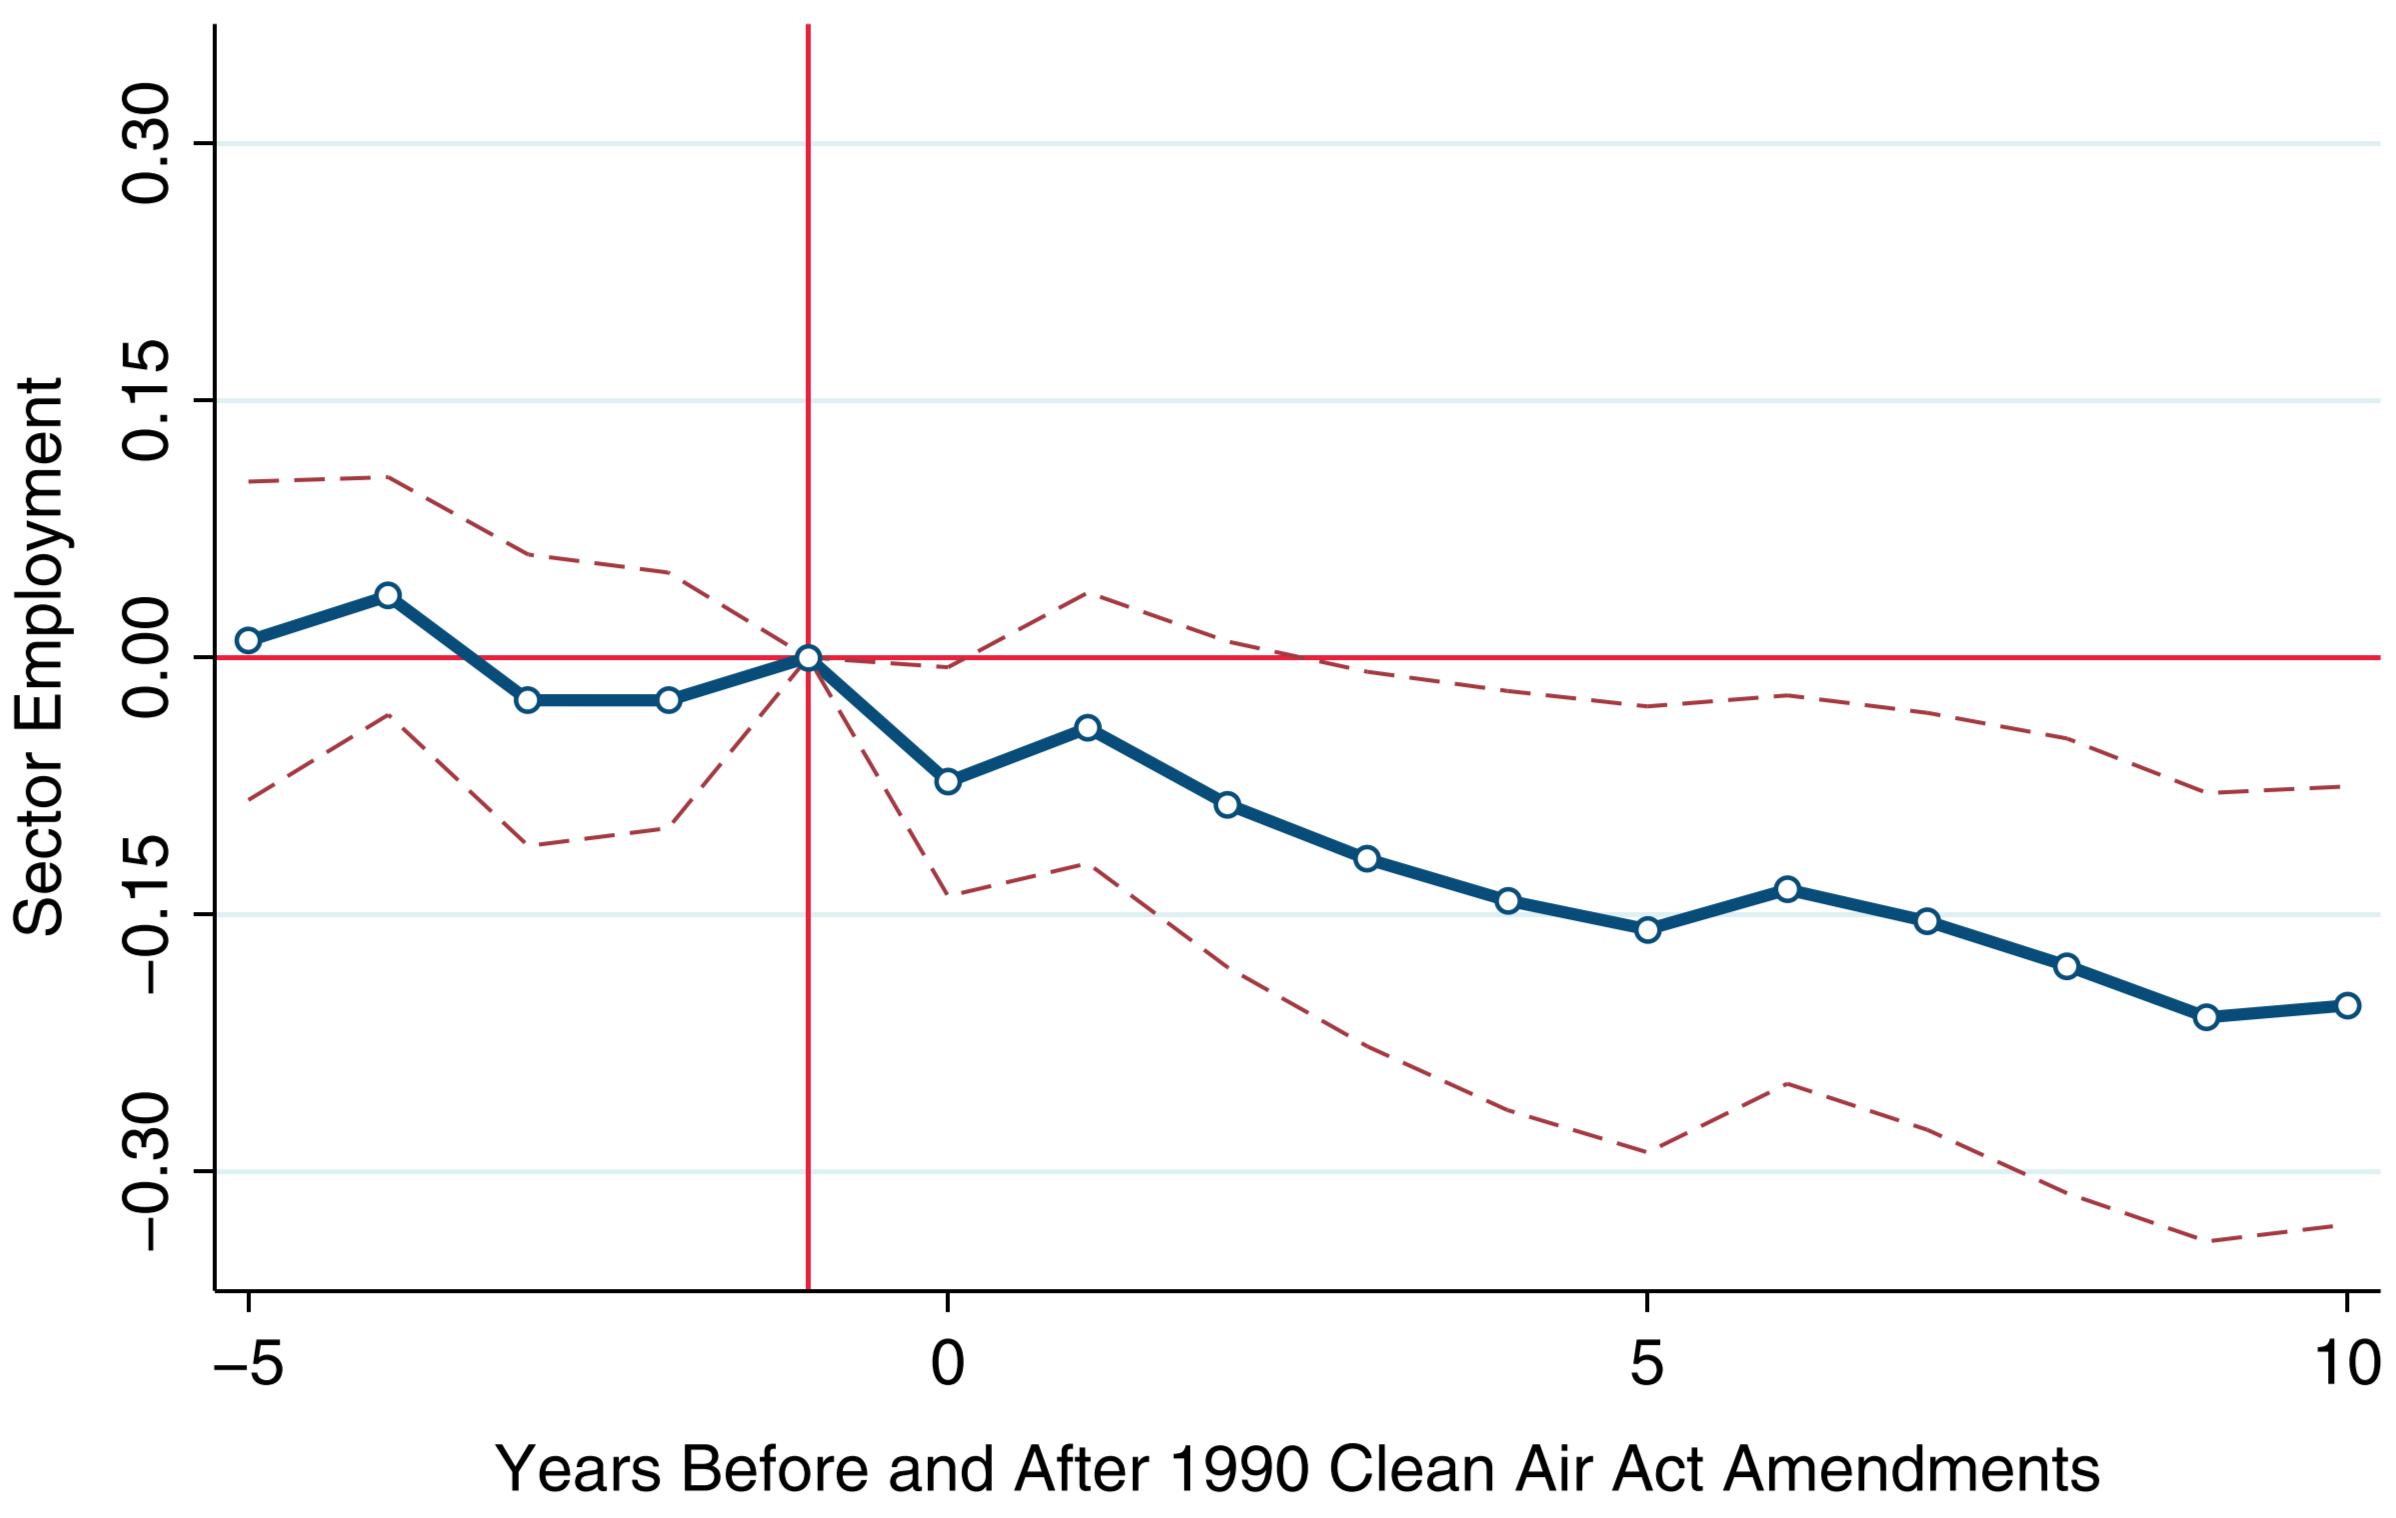
\includegraphics[scale=0.33]{figure2.png}
	\end{figure}
\end{frame}
%------------------------------------------------
\begin{frame}{B. The Wage Costs of Sectoral Reallocation: Evidence from Cohorts}
	\textbf{The central findings (using cohort earnings as the dpt variable):}
	\begin{figure}[h]
		\centering
		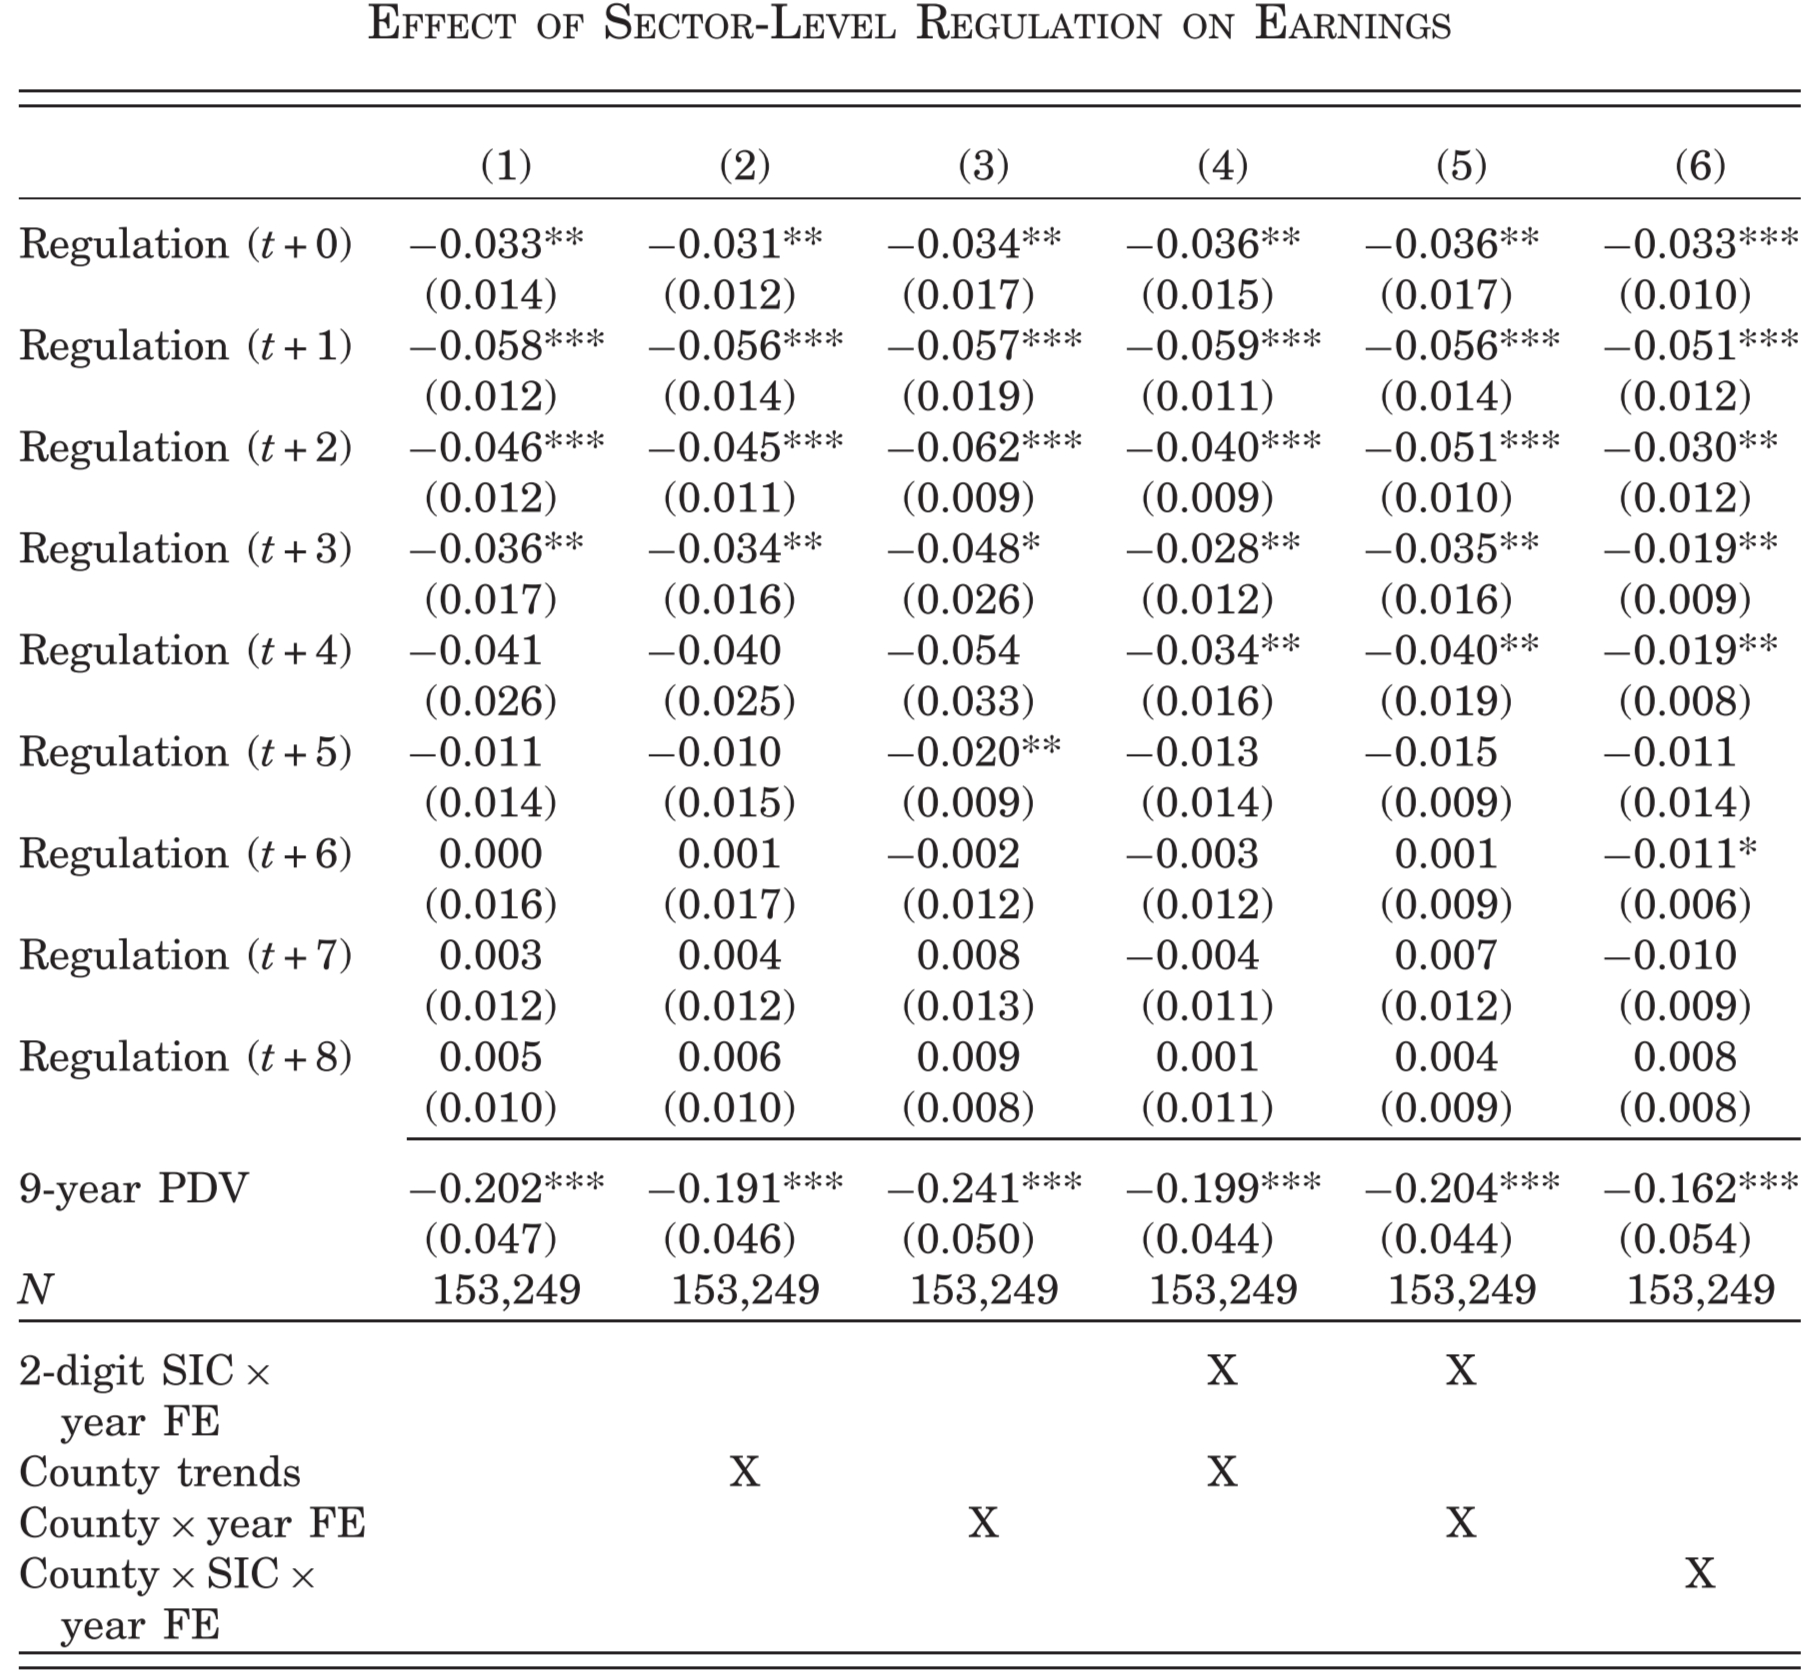
\includegraphics[scale=0.29]{table2.png}
	\end{figure}
\end{frame}
%------------------------------------------------
\begin{frame}[label=figure3]{B. The Wage Costs of Sectoral Reallocation: Evidence from Cohorts}
	\begin{figure}[h]
		\centering
		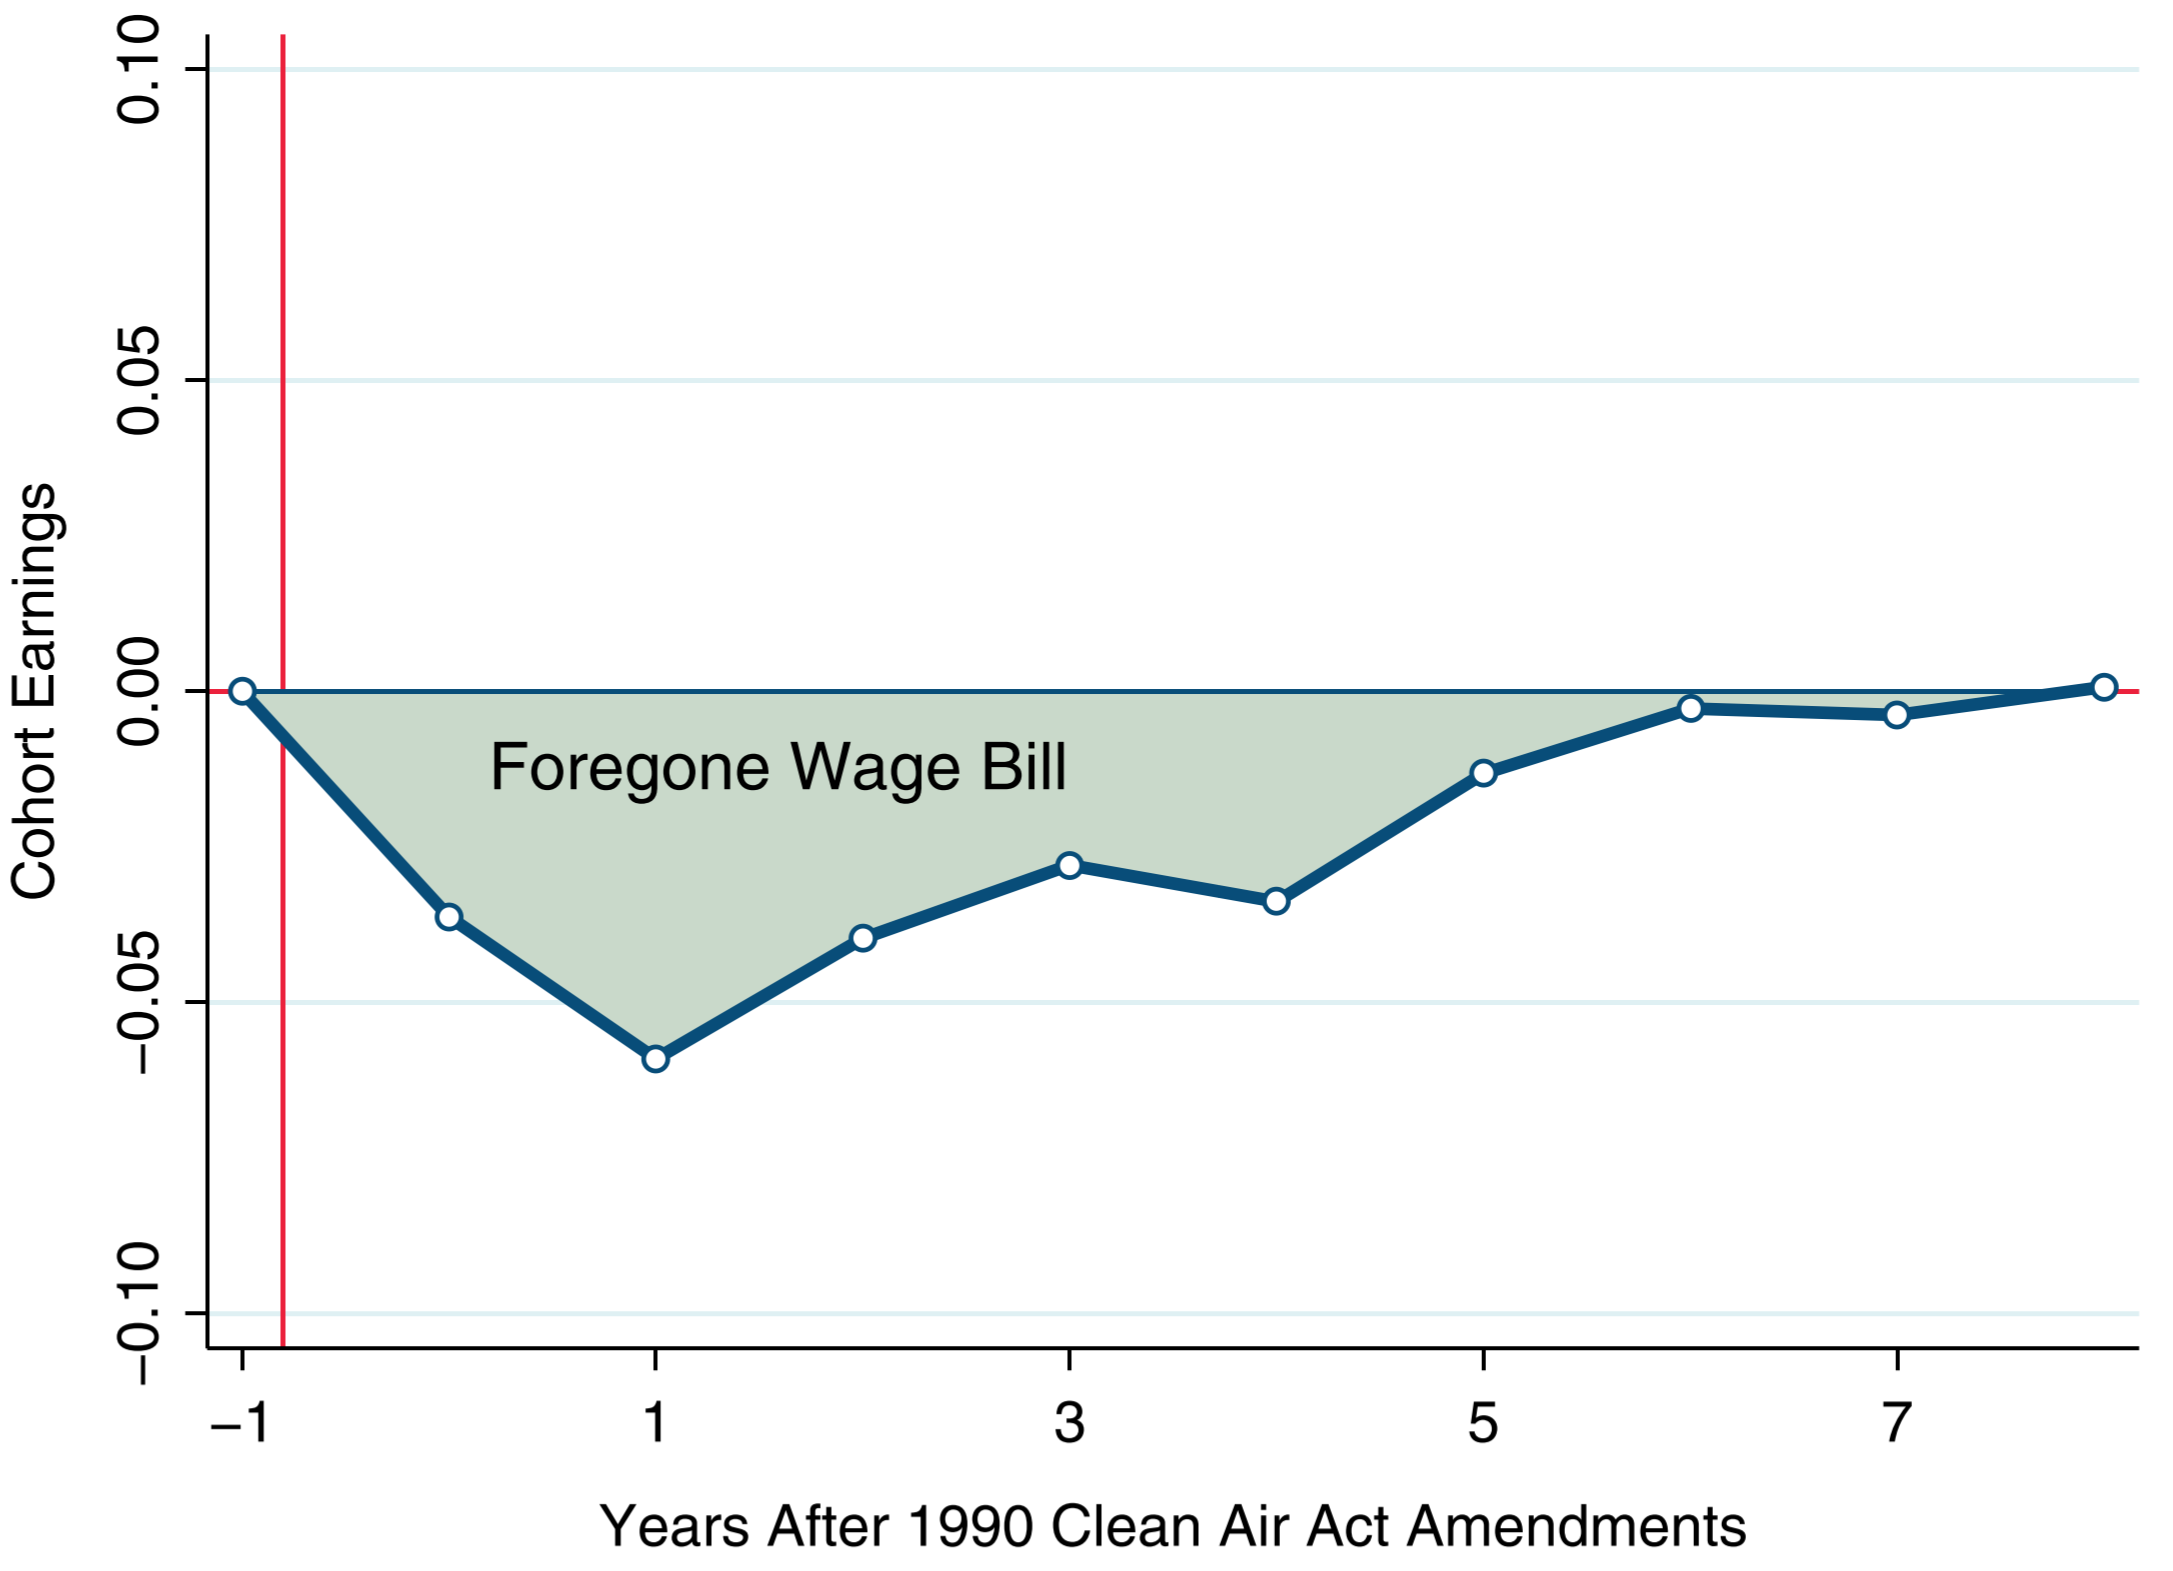
\includegraphics[scale=0.35]{figure3.png}
	\end{figure}
\end{frame}
%------------------------------------------------
\begin{frame}{B. The Wage Costs of Sectoral Reallocation: Evidence from Cohorts}
	Comparing the transitional dynamics between \textcolor{blue}{\hyperlink{figure2}{Figure 2}} and \textcolor{blue}{\hyperlink{figure3}{Figure 3}} to find that, \textcolor{red}{although employment trends in the newly regulated sector fall continuously in the years after the regulations go into place, the earnings dynamics initially fall and begin to recover in subsequent years.}
	\medskip

	Possible explanations for these seeming discrepancies:
	\begin{itemize}
		\item First, workers are \textcolor{red}{leaving the newly regulated sector}, which means that in the years following the policy, the employment "effect" on cohort earnings will be attenuated.
		\item Second, sectoral employment is measured \textcolor{red}{relative to a counterfactual}. It might be the case that employment is increasing in the counterfactual sector and remaining constant in the treated sector.
		\item Last, another important factor underlying the magnitude and duration of the earnings losses is \textcolor{red}{the underlying condition of the aggregate and local labor market in early versus later years of the sample}.
	\end{itemize}
\end{frame}
%------------------------------------------------
\begin{frame}{C. Effects of Regulations for "Stayers" and "Leavers"}
	\textbf{heterogeneity:} Here, I decompose the earnings changes into \textcolor{red}{the component explained by workers that remain with their initial employer} and \textcolor{red}{the component explained by workers who separate from their initial employer}.\footnote{The earnings of the various control group cohorts remain the same as in the previous section, whereas the newly regulated sector's earnings consists only of stayers or only of leavers, depending on the specification.}
\end{frame}
%------------------------------------------------
\begin{frame}{C. Effects of Regulations for "Stayers" and "Leavers"}
	\begin{figure}[h]
		\centering
		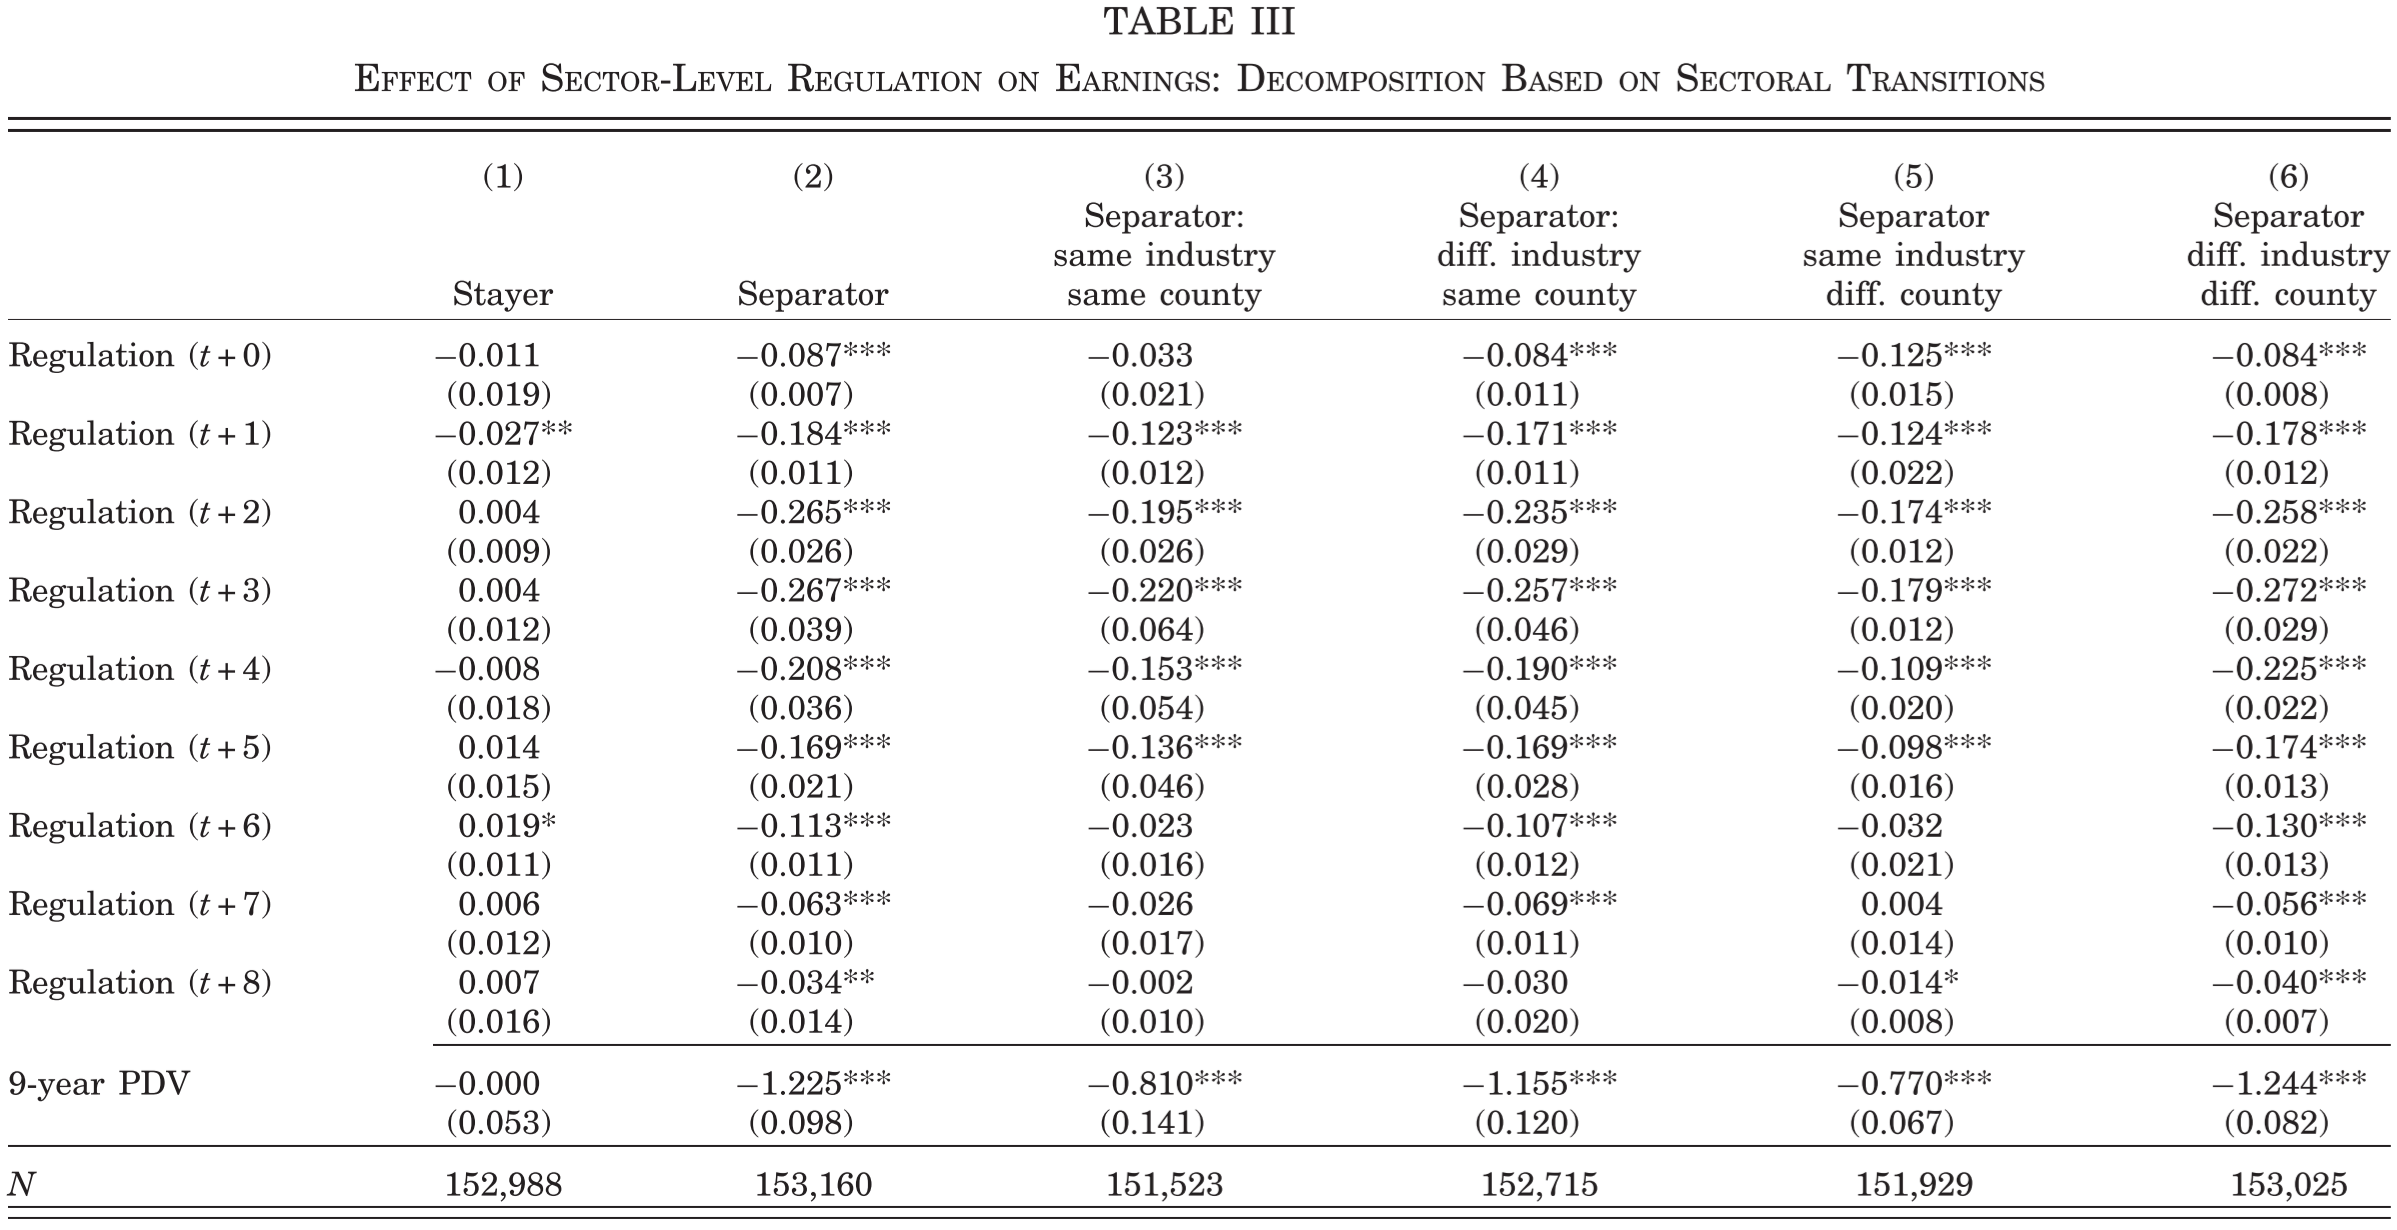
\includegraphics[scale=0.37]{table3.png}
	\end{figure}
\end{frame}
%------------------------------------------------
\begin{frame}{C. Effects of Regulations for "Stayers" and "Leavers"}
	In general, the earnings loss attributable to job separations in this context is \textcolor{red}{smaller than} estimates found in the literature on displacement induced by mass layoffs. Notably,the earnings recovery of the average worker in this setting is \textcolor{red}{more rapid than} that found in the displacement literature.
	\medskip

	A few possible explanations for these discrepancies.
	\begin{enumerate}
		\item It seems possible that the rapid earnings recovery comes from the fact that \textcolor{red}{most of these regulations occur in dense, urban labor markets}.
		\item It is possible that some of the job transitions I observe \textcolor{red}{a revoluntary, job-to-job transitions for which workers often experience a rise in earnings}.
		\item The rapid earnings recovery may be unique to this setting, \textcolor{red}{stemming from the high-pressure labor market in the mid-to-late 1990s}.
		\item An alternative explanation for this relatively quick recovery comes from the \textcolor{red}{difference in research designs and research questions}.
	\end{enumerate}
\end{frame}
%------------------------------------------------
\begin{frame}{C. Effects of Regulations for "Stayers" and "Leavers"}
	\begin{figure}[h]
		\centering
		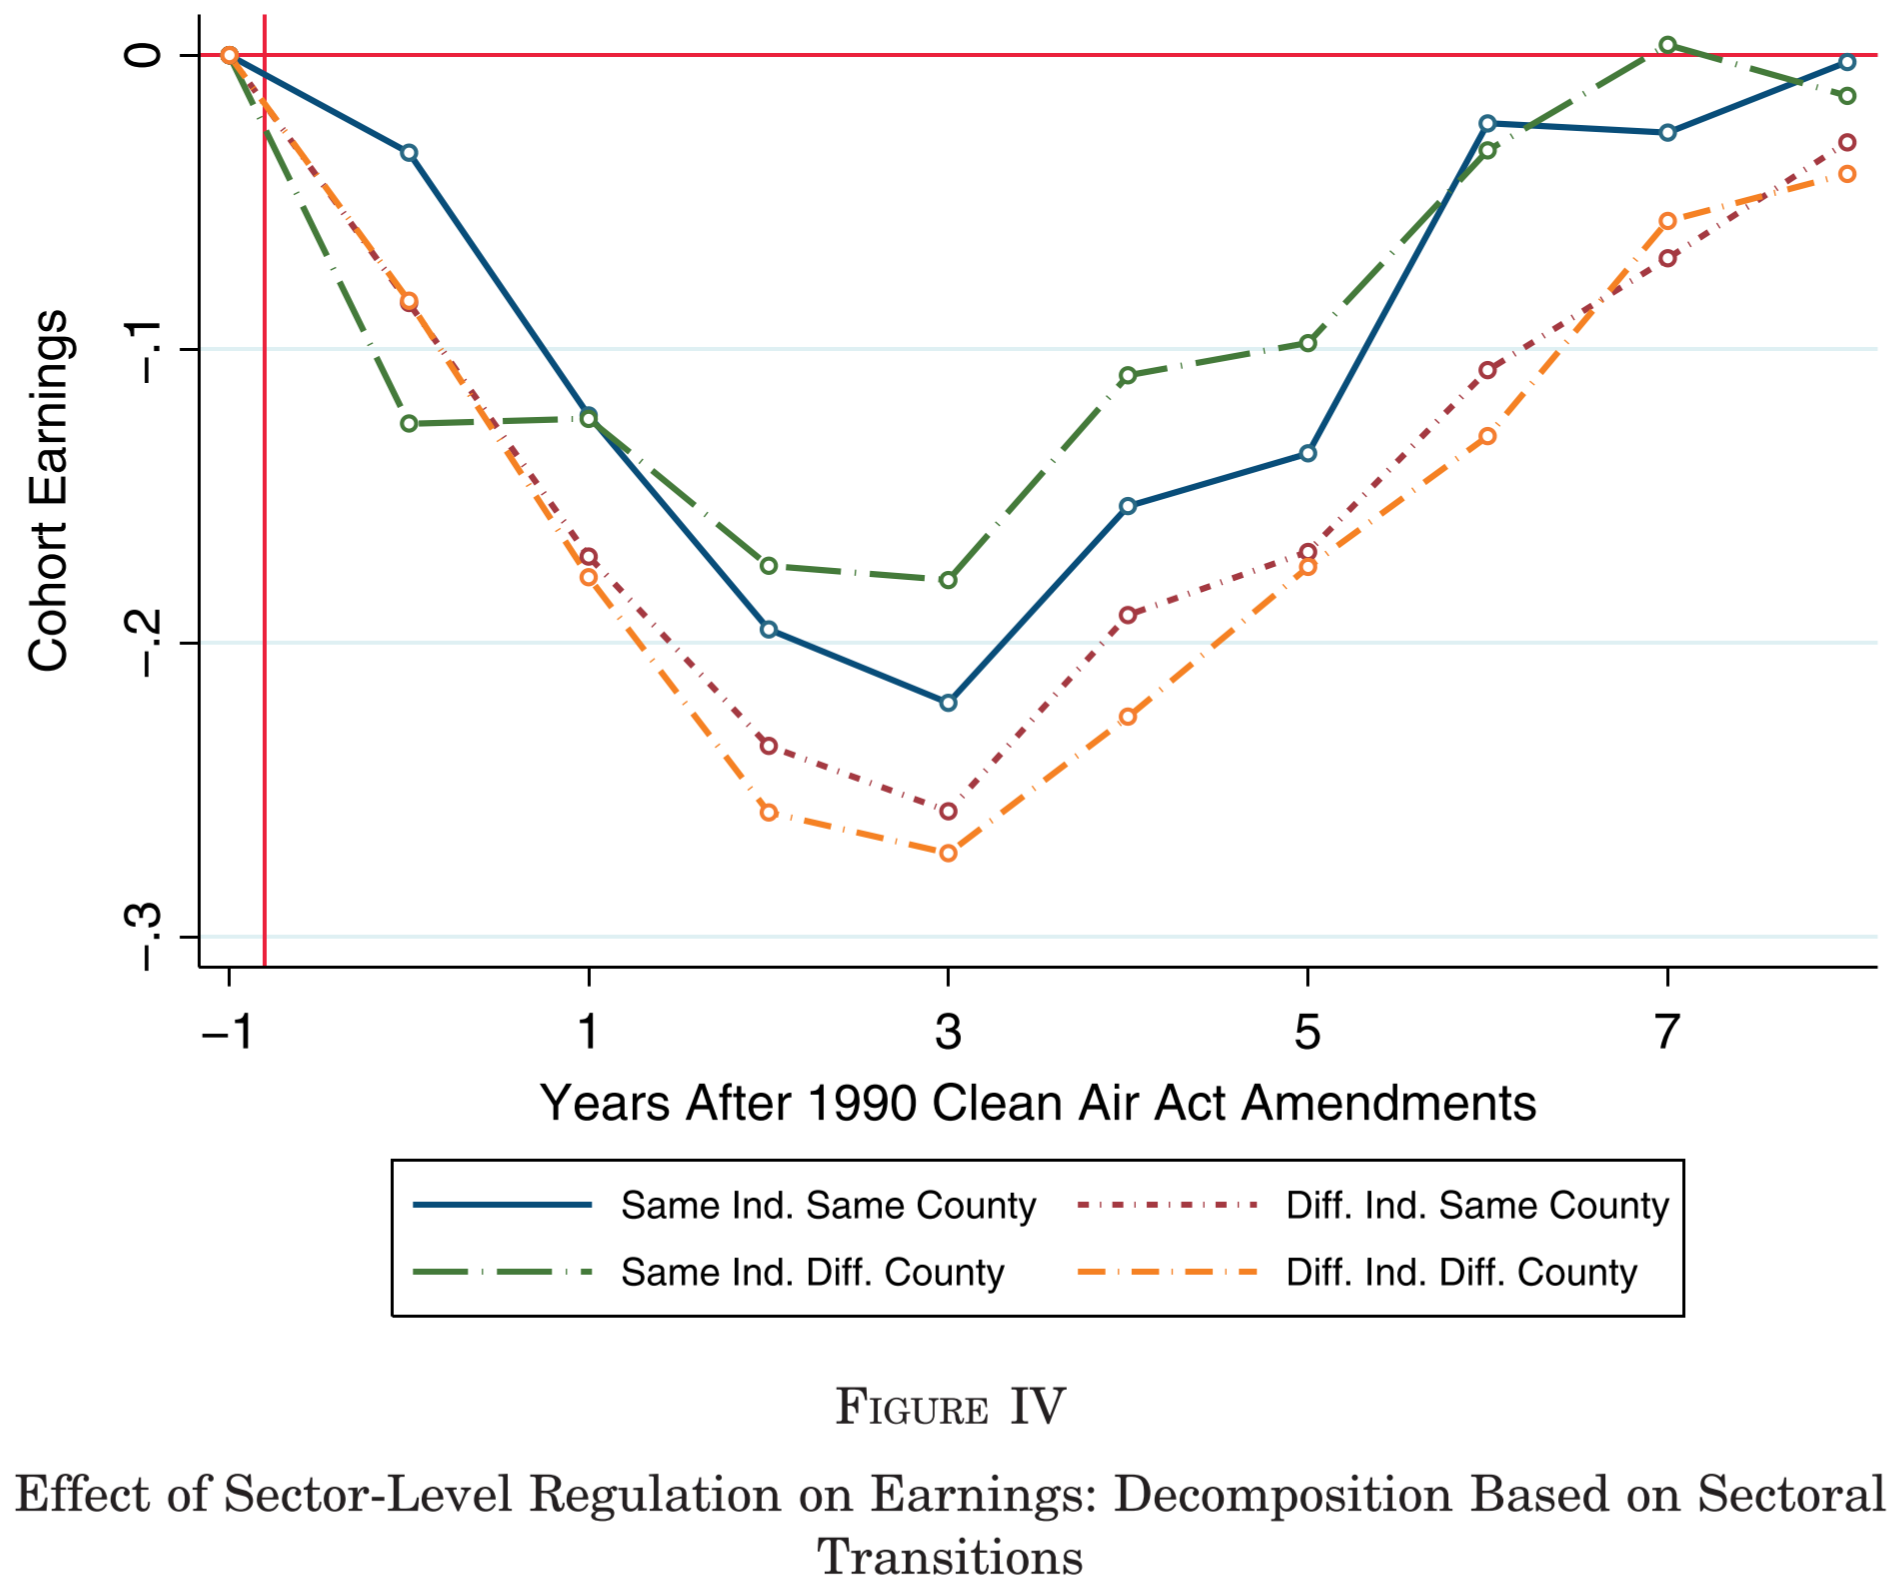
\includegraphics[scale=0.37]{figure4.png}
	\end{figure}
\end{frame}
%------------------------------------------------
\begin{frame}{D.Heterogeneity and Robustness of Cohort Wage Estimates}
	\begin{figure}[h]
		\centering
		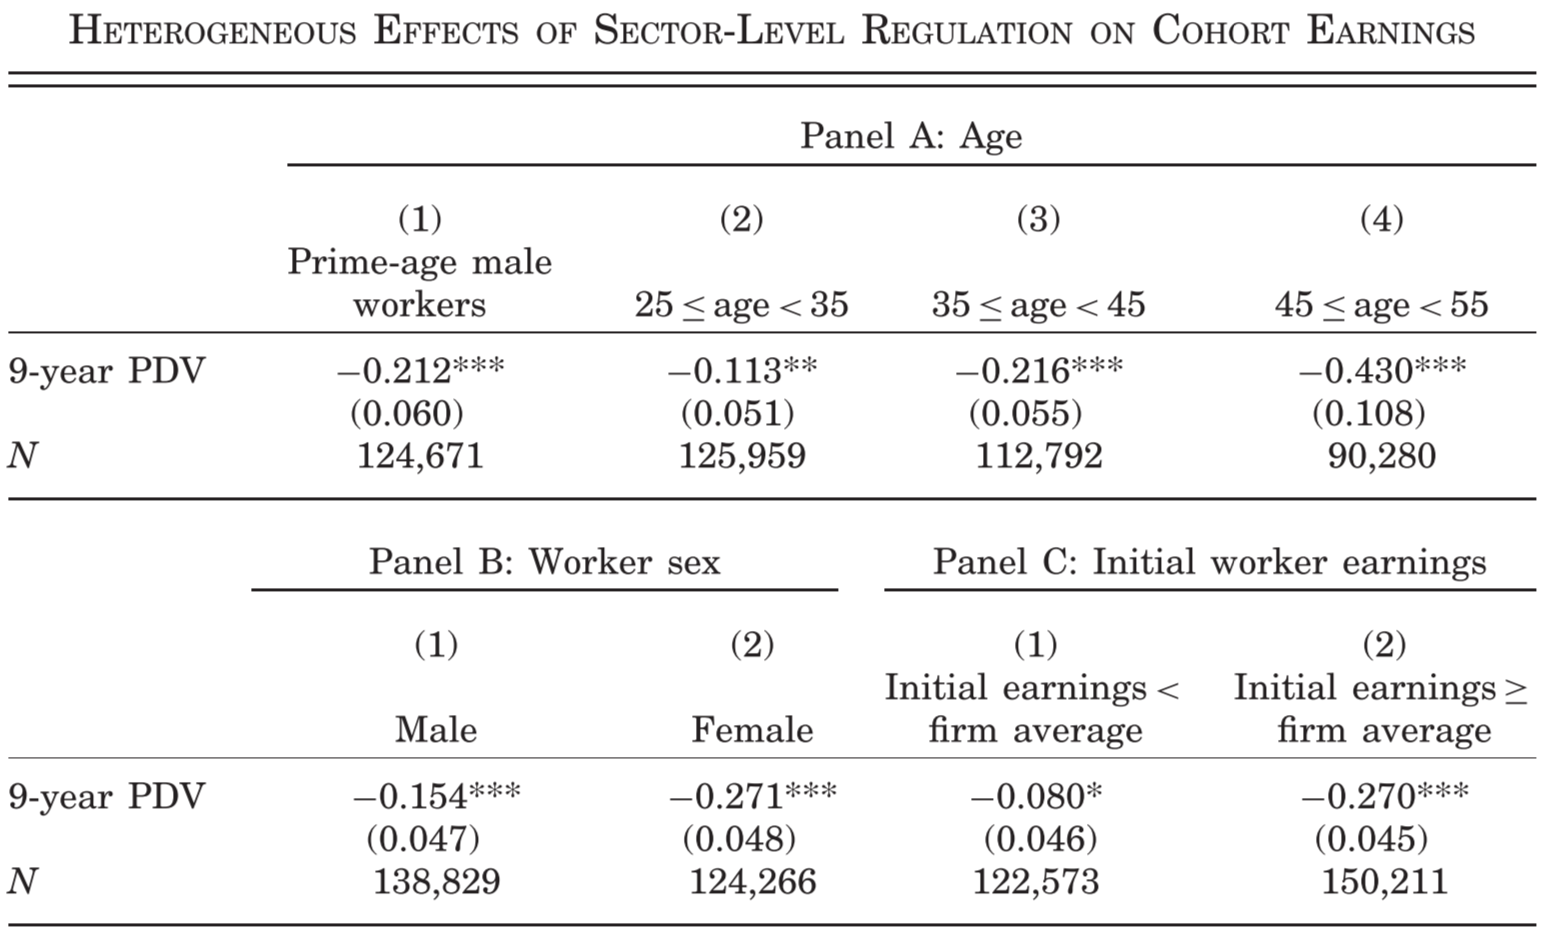
\includegraphics[scale=0.55]{table4_1.png}
	\end{figure}
\end{frame}
%------------------------------------------------
\begin{frame}{D.Heterogeneity and Robustness of Cohort Wage Estimates}
	\begin{figure}[h]
		\centering
		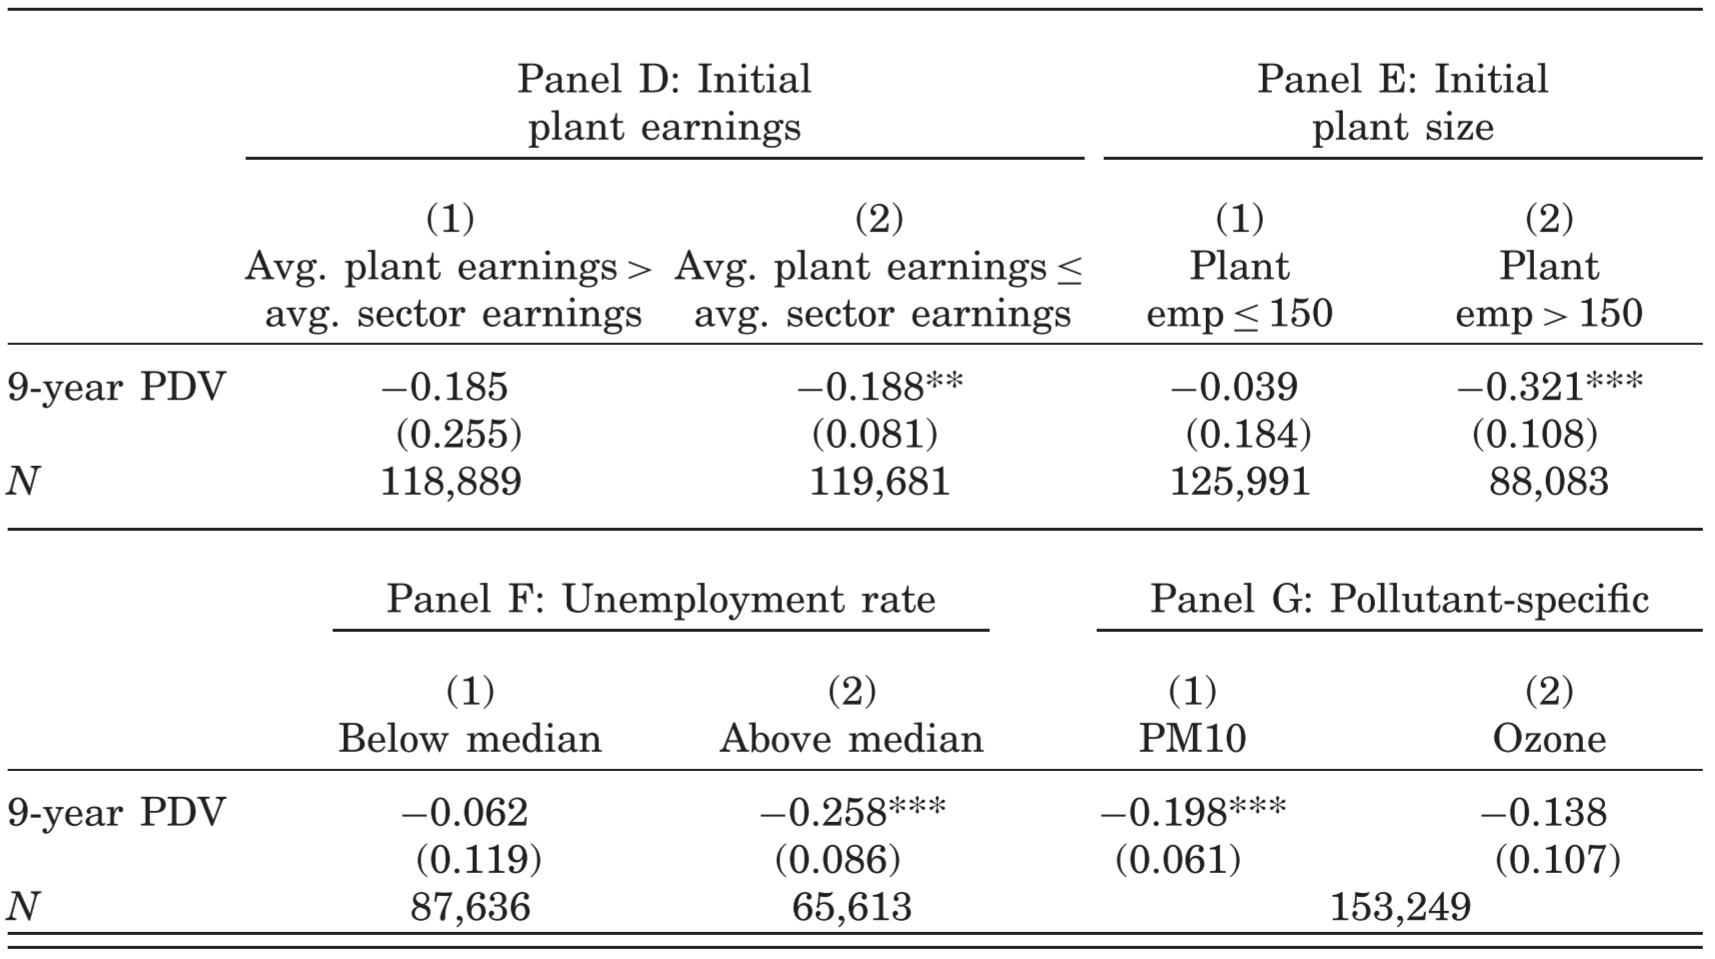
\includegraphics[scale=0.5]{table4_2.png}
	\end{figure}
\end{frame}
%------------------------------------------------
\begin{frame}{D.Heterogeneity and Robustness of Cohort Wage Estimates}{1. The Heterogeneous Impacts of Nonattainment within the	Earnings Distribution}
	\textbf{Percentile regression of the earnings distribution}
	\begin{itemize}
		\item I begin by calculating the 1st, 5th, 10th, 25th, 50th, 75th, 90th, 95th, and 99th percentiles of the within-cohort, pretreatment earnings distribution.
		\item For each subsequent, post-CAAA year, I classify individuals into bins based on their place in the "pretreatment" earnings distribution.
		\item Collapsing the data to the cohort-year yields the fraction of individuals in a given cohort that are in the binned percentile of the 1990 earnings distribution.
		\item An increase in the binned percentile variable would mean that the regulations led to a relative increase in the fraction of individuals in this part of earnings distribution.
	\end{itemize}
\end{frame}
%------------------------------------------------
\begin{frame}{D.Heterogeneity and Robustness of Cohort Wage Estimates}{1. The Heterogeneous Impacts of Nonattainment within the	Earnings Distribution}
	\textbf{Percentile regression of the earnings distribution}
	\begin{figure}[h]
		\centering
		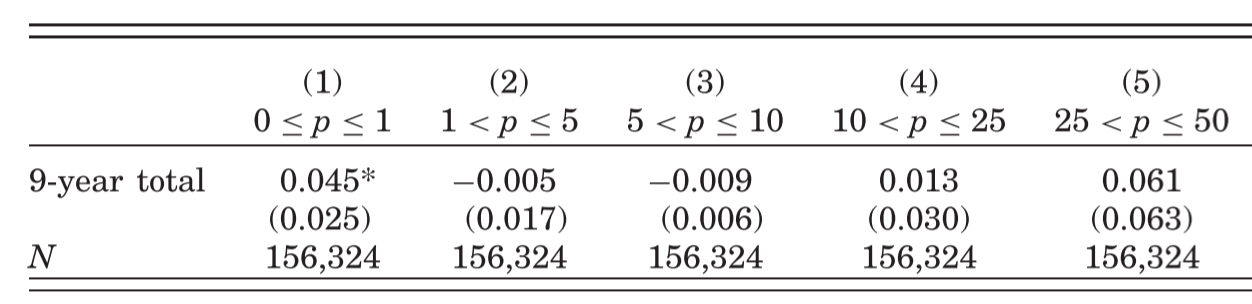
\includegraphics[scale=0.7]{table5_1.png}
		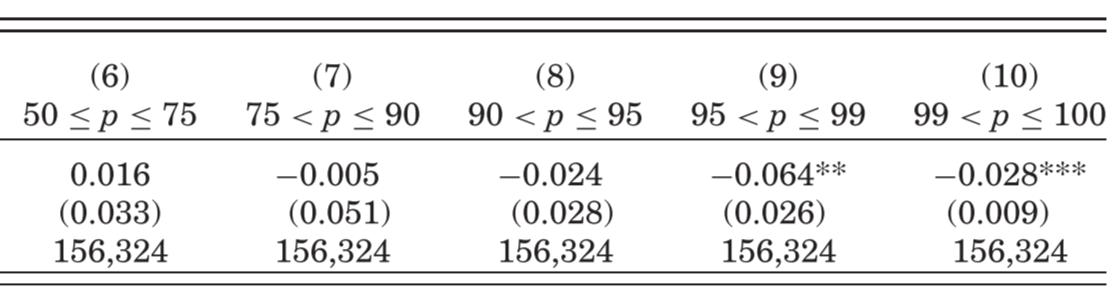
\includegraphics[scale=0.7]{table5_2.png}
	\end{figure}
\end{frame}
%------------------------------------------------
\begin{frame}{D.Heterogeneity and Robustness of Cohort Wage Estimates}{2. Local Labor Market Spillovers and Additional Specifications}
	Previous results showed that when we isolate the source of identifying variation to come from \textit{within} a county$\times$industry$\times$year, the regression estimates are somewhat \textcolor{red}{attenuated} relative to estimates that use both within- and across-county variation for identification.
	\medskip

	Part of this result may have to do with \textcolor{red}{spillovers in the local labor market} and \textcolor{red}{"contamination" of the control group}.
	\begin{itemize}
		\item If workers disproportionately find new jobs within the same county, this could put pressure on earnings in "counterfactual" sectors (i.e., by pushing out the labor supply curve).
		\item Additional tests show that the labor market contamination effects in the "within-county" control group are small.
	\end{itemize}
\end{frame}
%------------------------------------------------
\begin{frame}{E. Mechanisms: Regulation Increases the Separation Rate and Time between Jobs}
	\textbf{Probe into how job flow dynamics interact with the underlying cohort earnings regressions:} estimate the degree to which changes in environmental regulations lead to excess labor reallocation in the years following the policy.
	\medskip

	The empirical analysis estimates how this failure rate changes as a function of the new environmental regulations. \textcolor{blue}{\hyperlink{figure5}{Figure V}} plots estimates of the $\eta_1^k$'s from equation (2), with \textcolor{red}{the dpt variable the failure rate for the newly regulated sector}.
\end{frame}
%------------------------------------------------
\begin{frame}[label=figure5]{E. Mechanisms: Regulation Increases the Separation Rate and Time between Jobs}
	\begin{figure}[h]
		\centering
		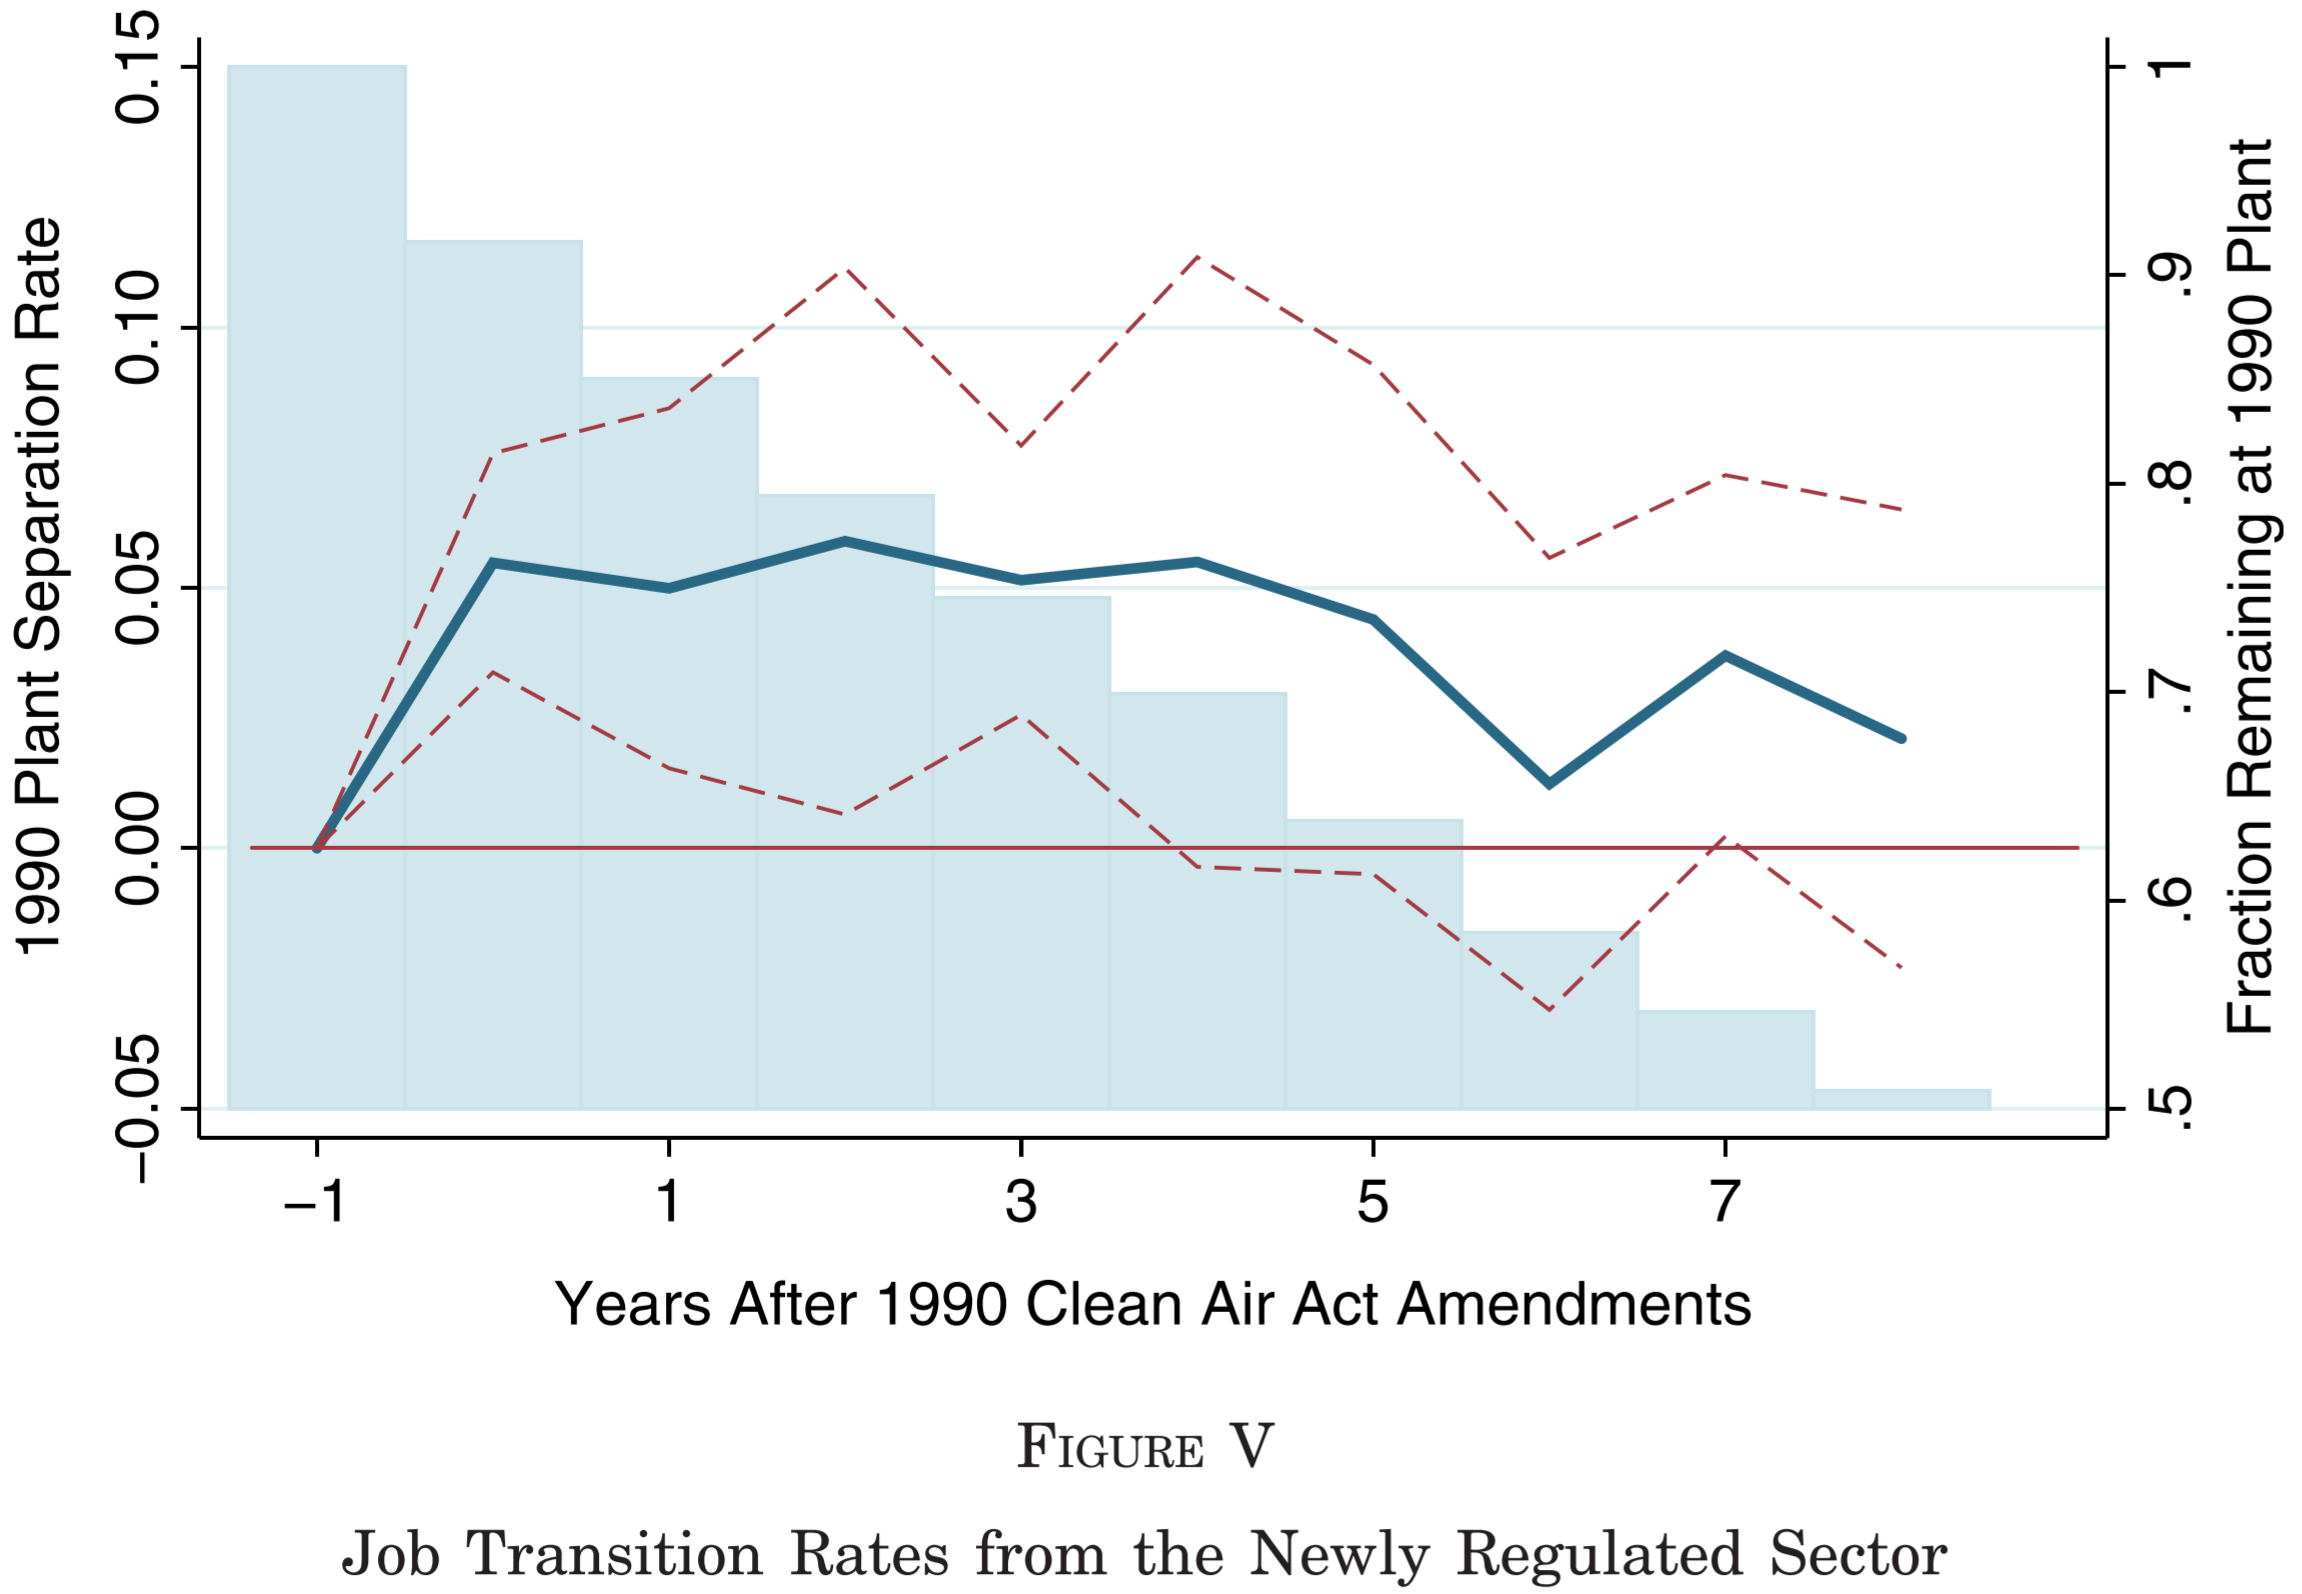
\includegraphics[scale=0.35]{figure5.png}
	\end{figure}
\end{frame}
%------------------------------------------------
\begin{frame}{E. Mechanisms: Regulation Increases the Separation Rate and Time between Jobs}
	\begin{figure}[h]
		\centering
		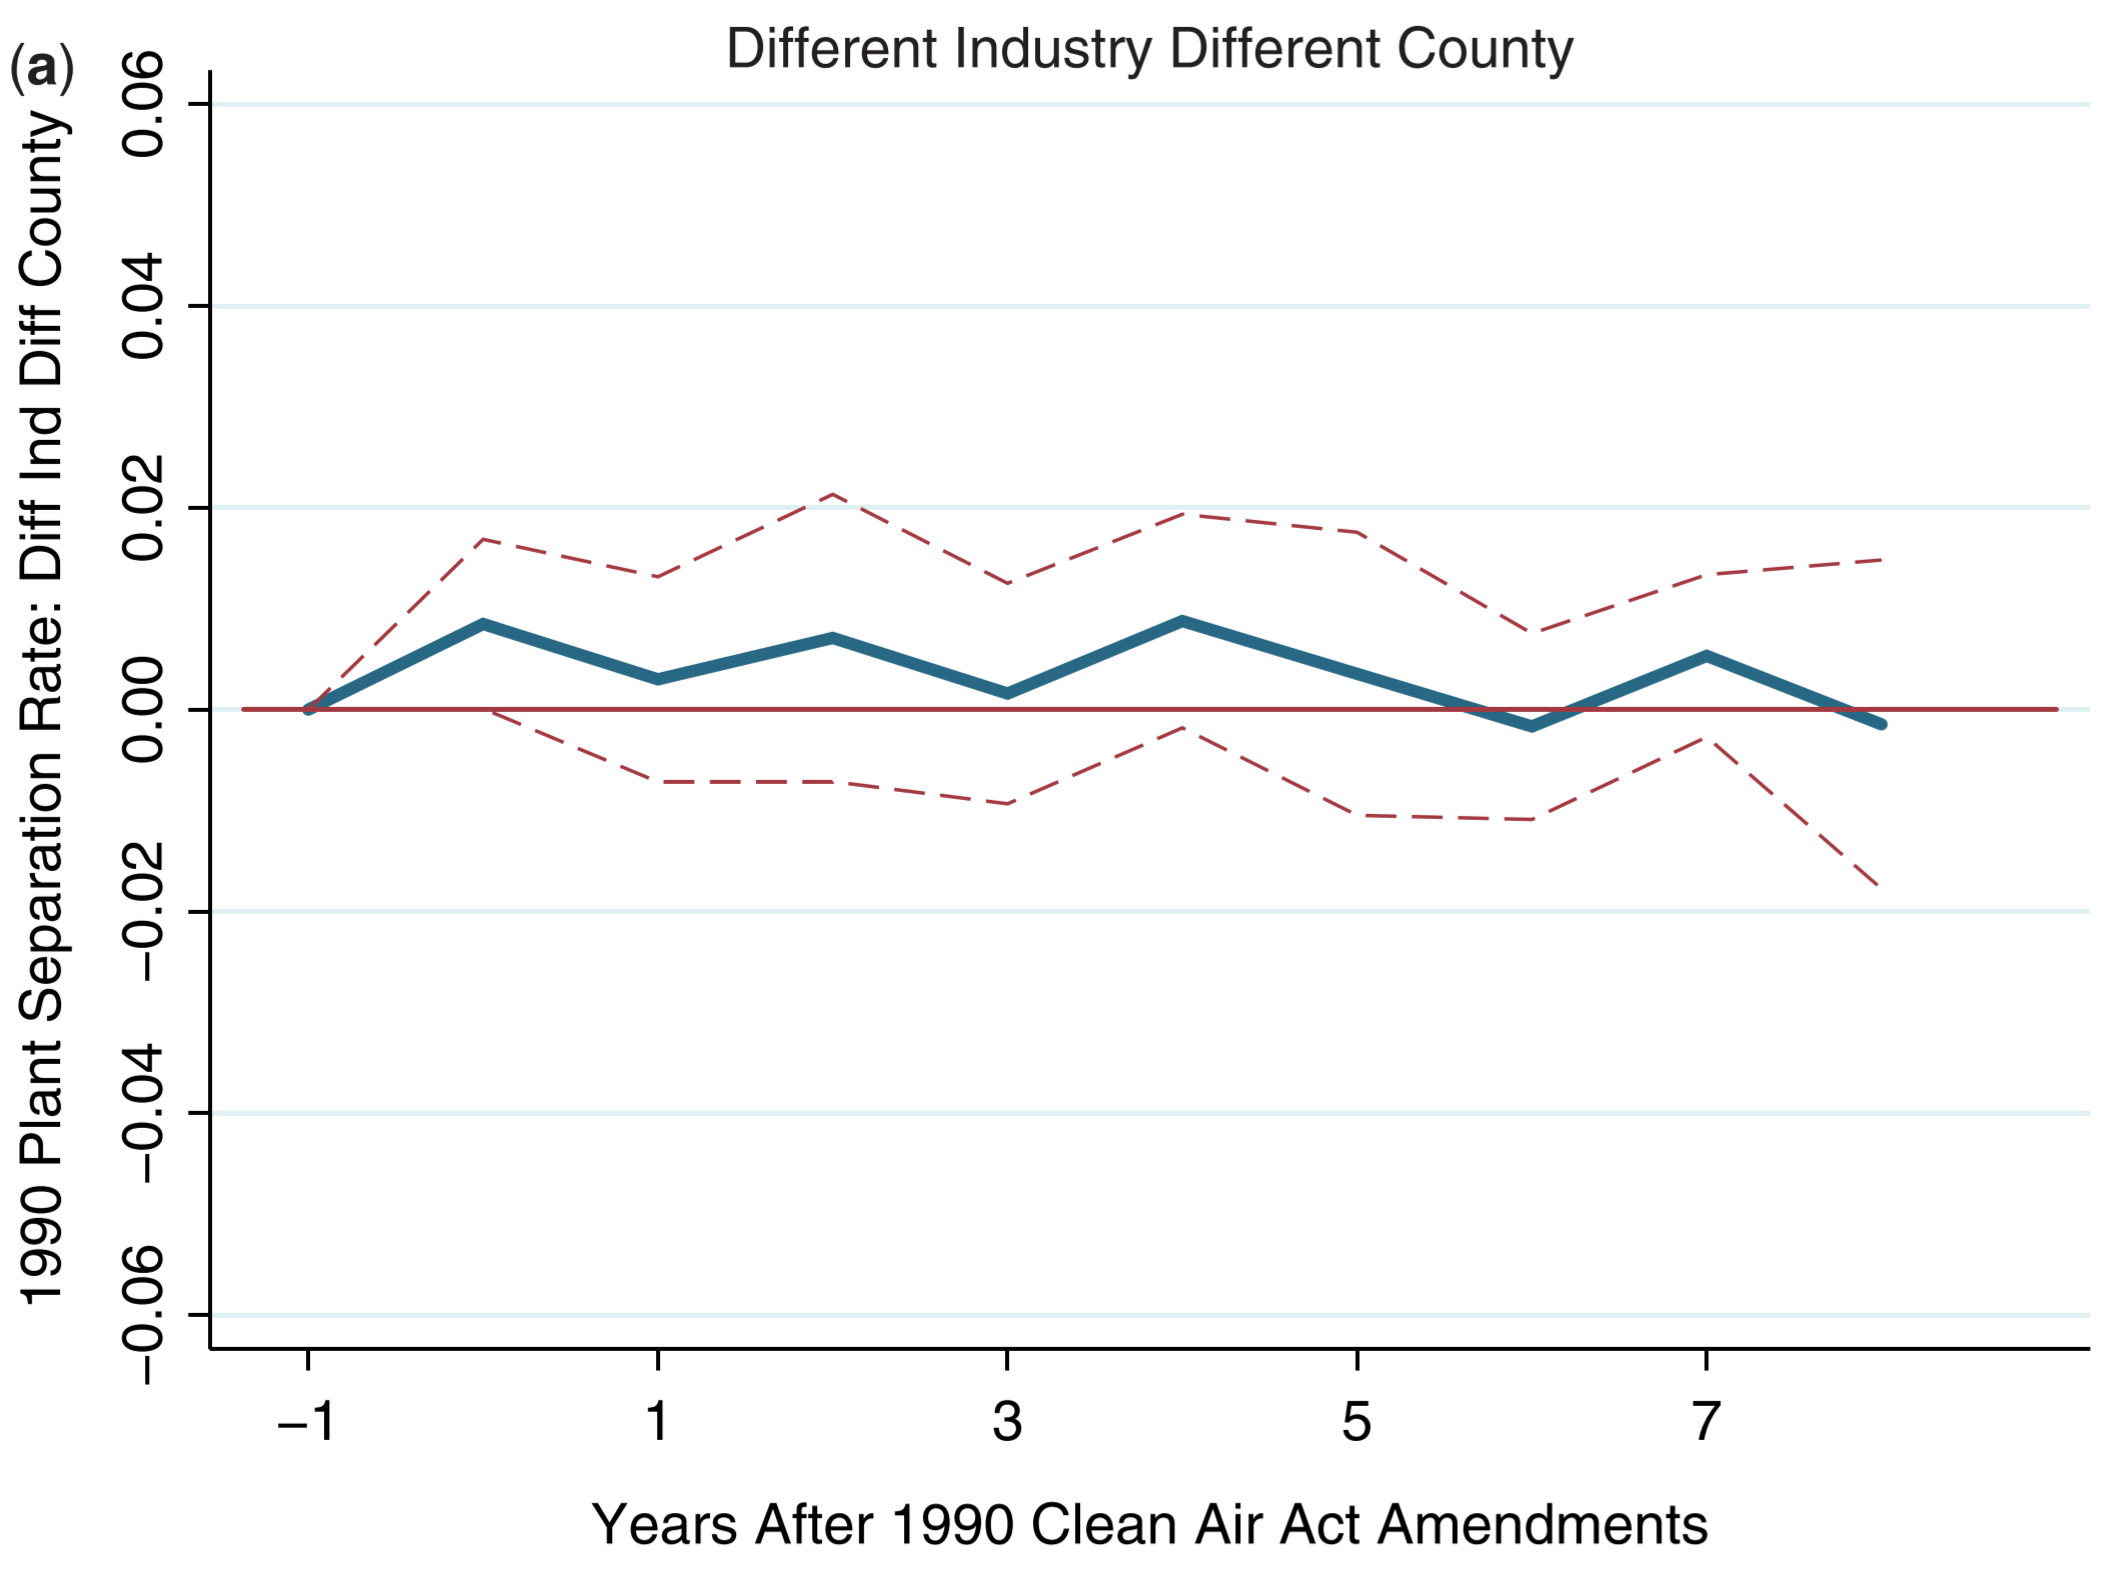
\includegraphics[scale=0.35]{figure6a.png}
	\end{figure}
\end{frame}
%------------------------------------------------
\begin{frame}{E. Mechanisms: Regulation Increases the Separation Rate and Time between Jobs}
	\begin{figure}[h]
		\centering
		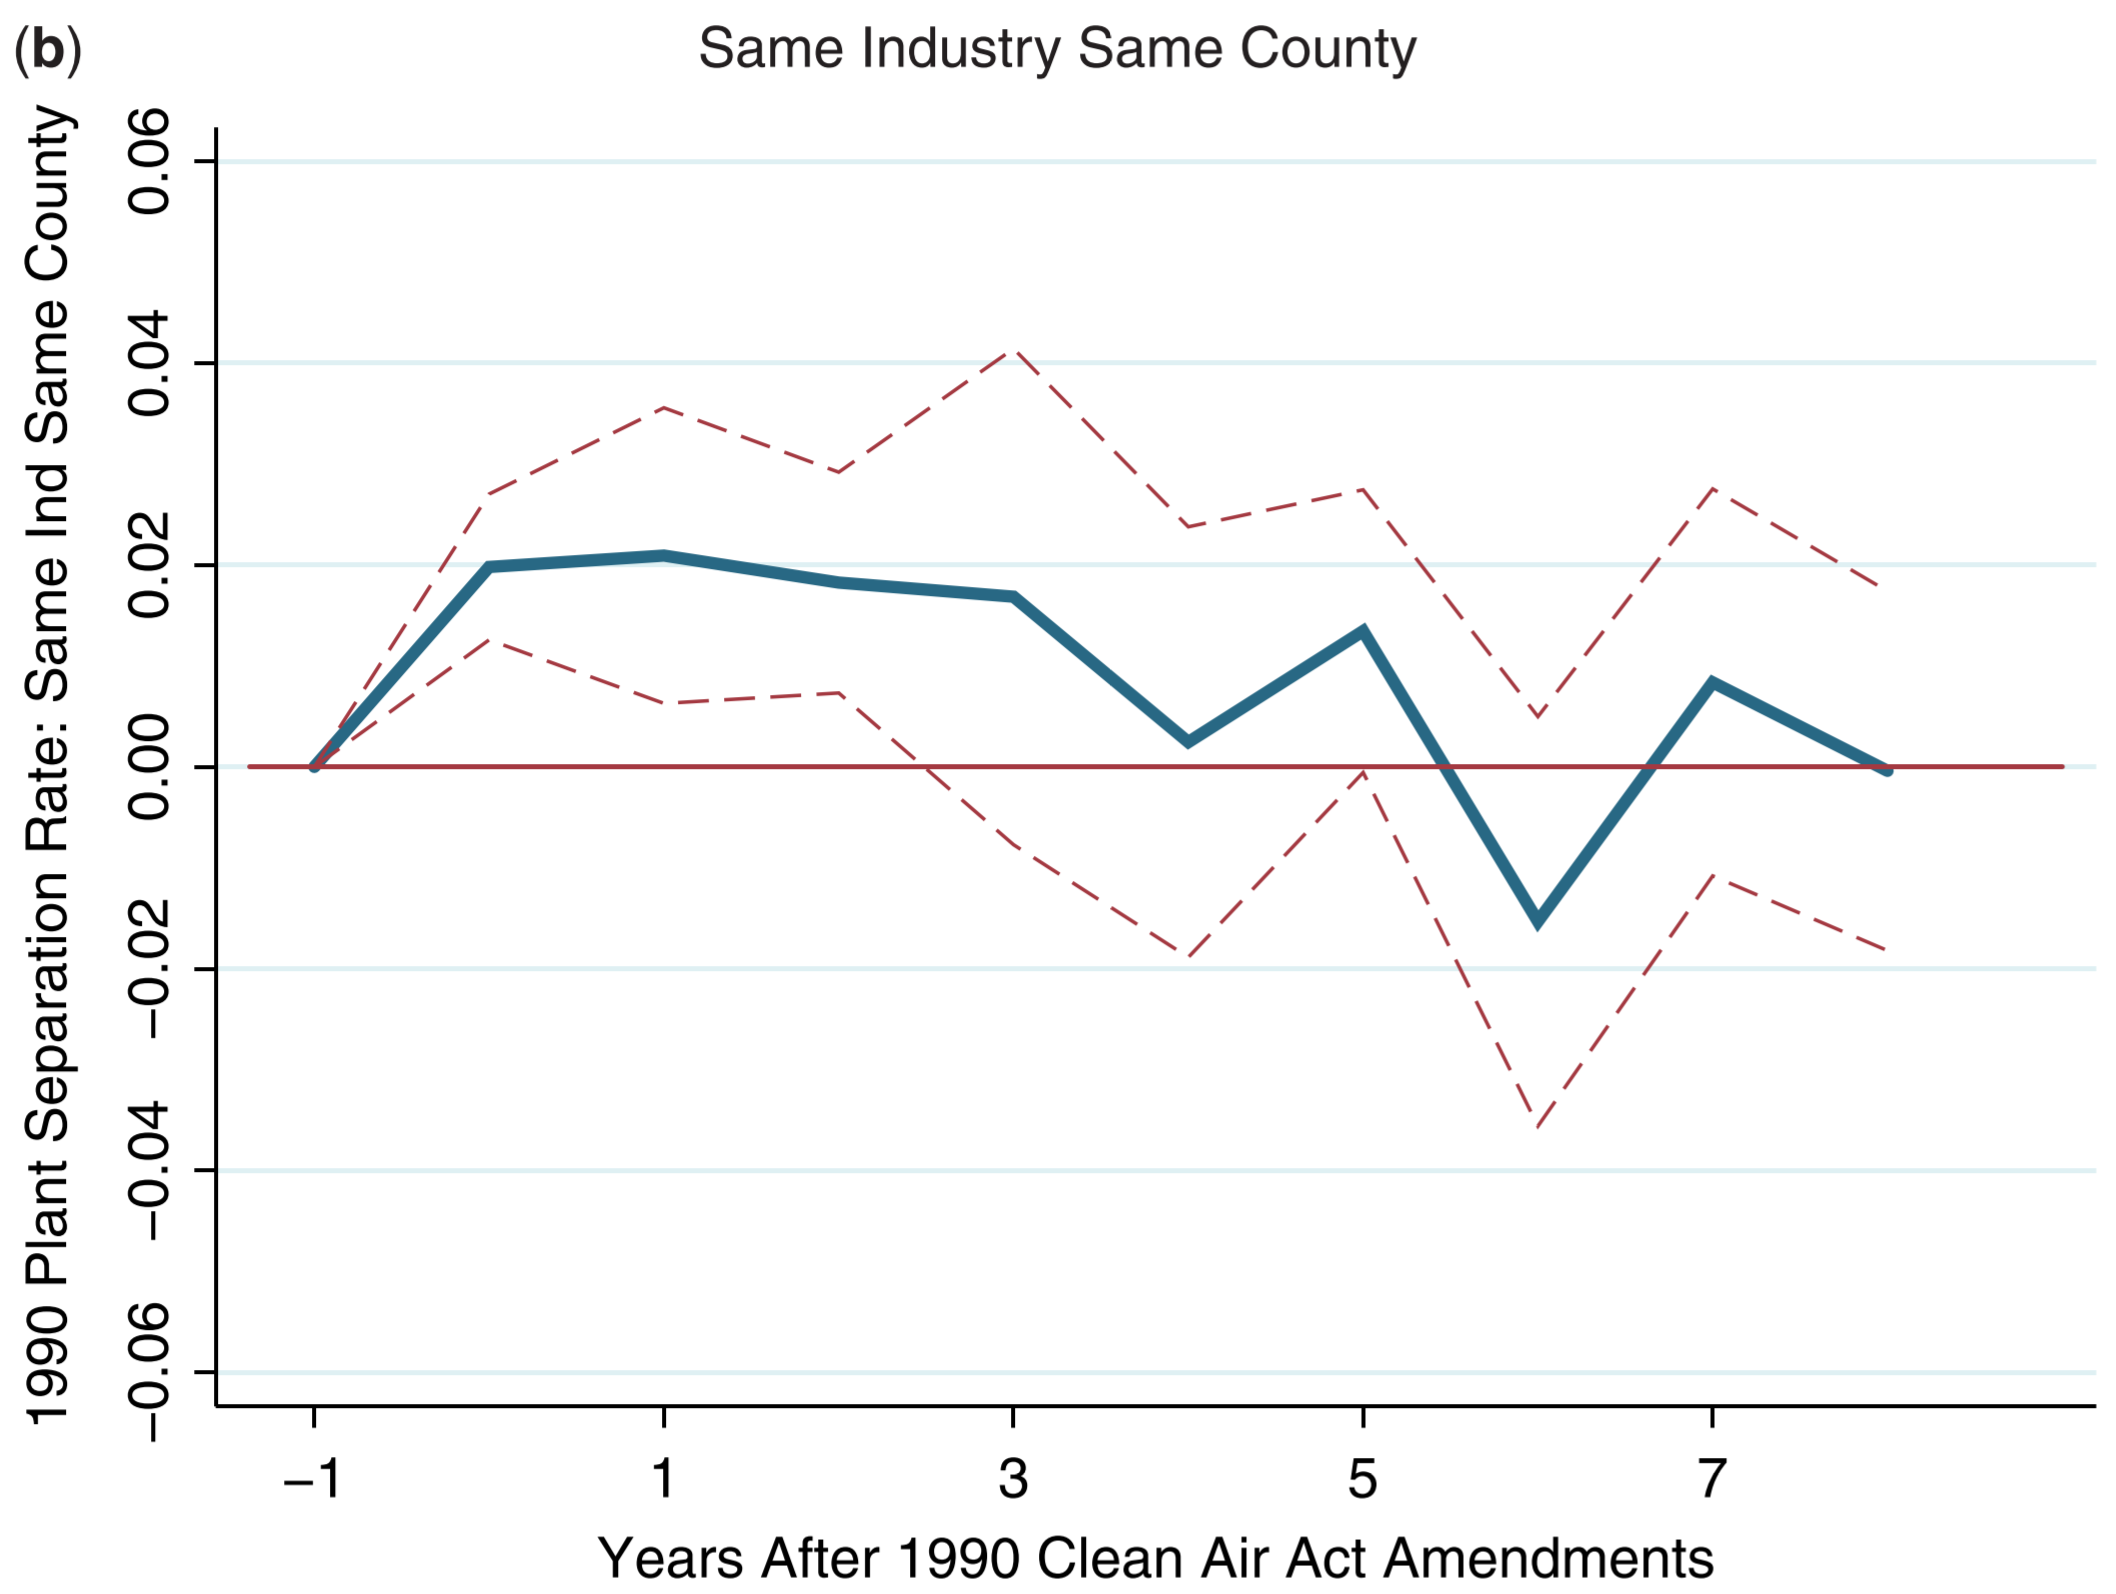
\includegraphics[scale=0.35]{figure6b.png}
	\end{figure}
\end{frame}
%------------------------------------------------
\begin{frame}{E. Mechanisms: Regulation Increases the Separation Rate and Time between Jobs}
	\begin{figure}[h]
		\centering
		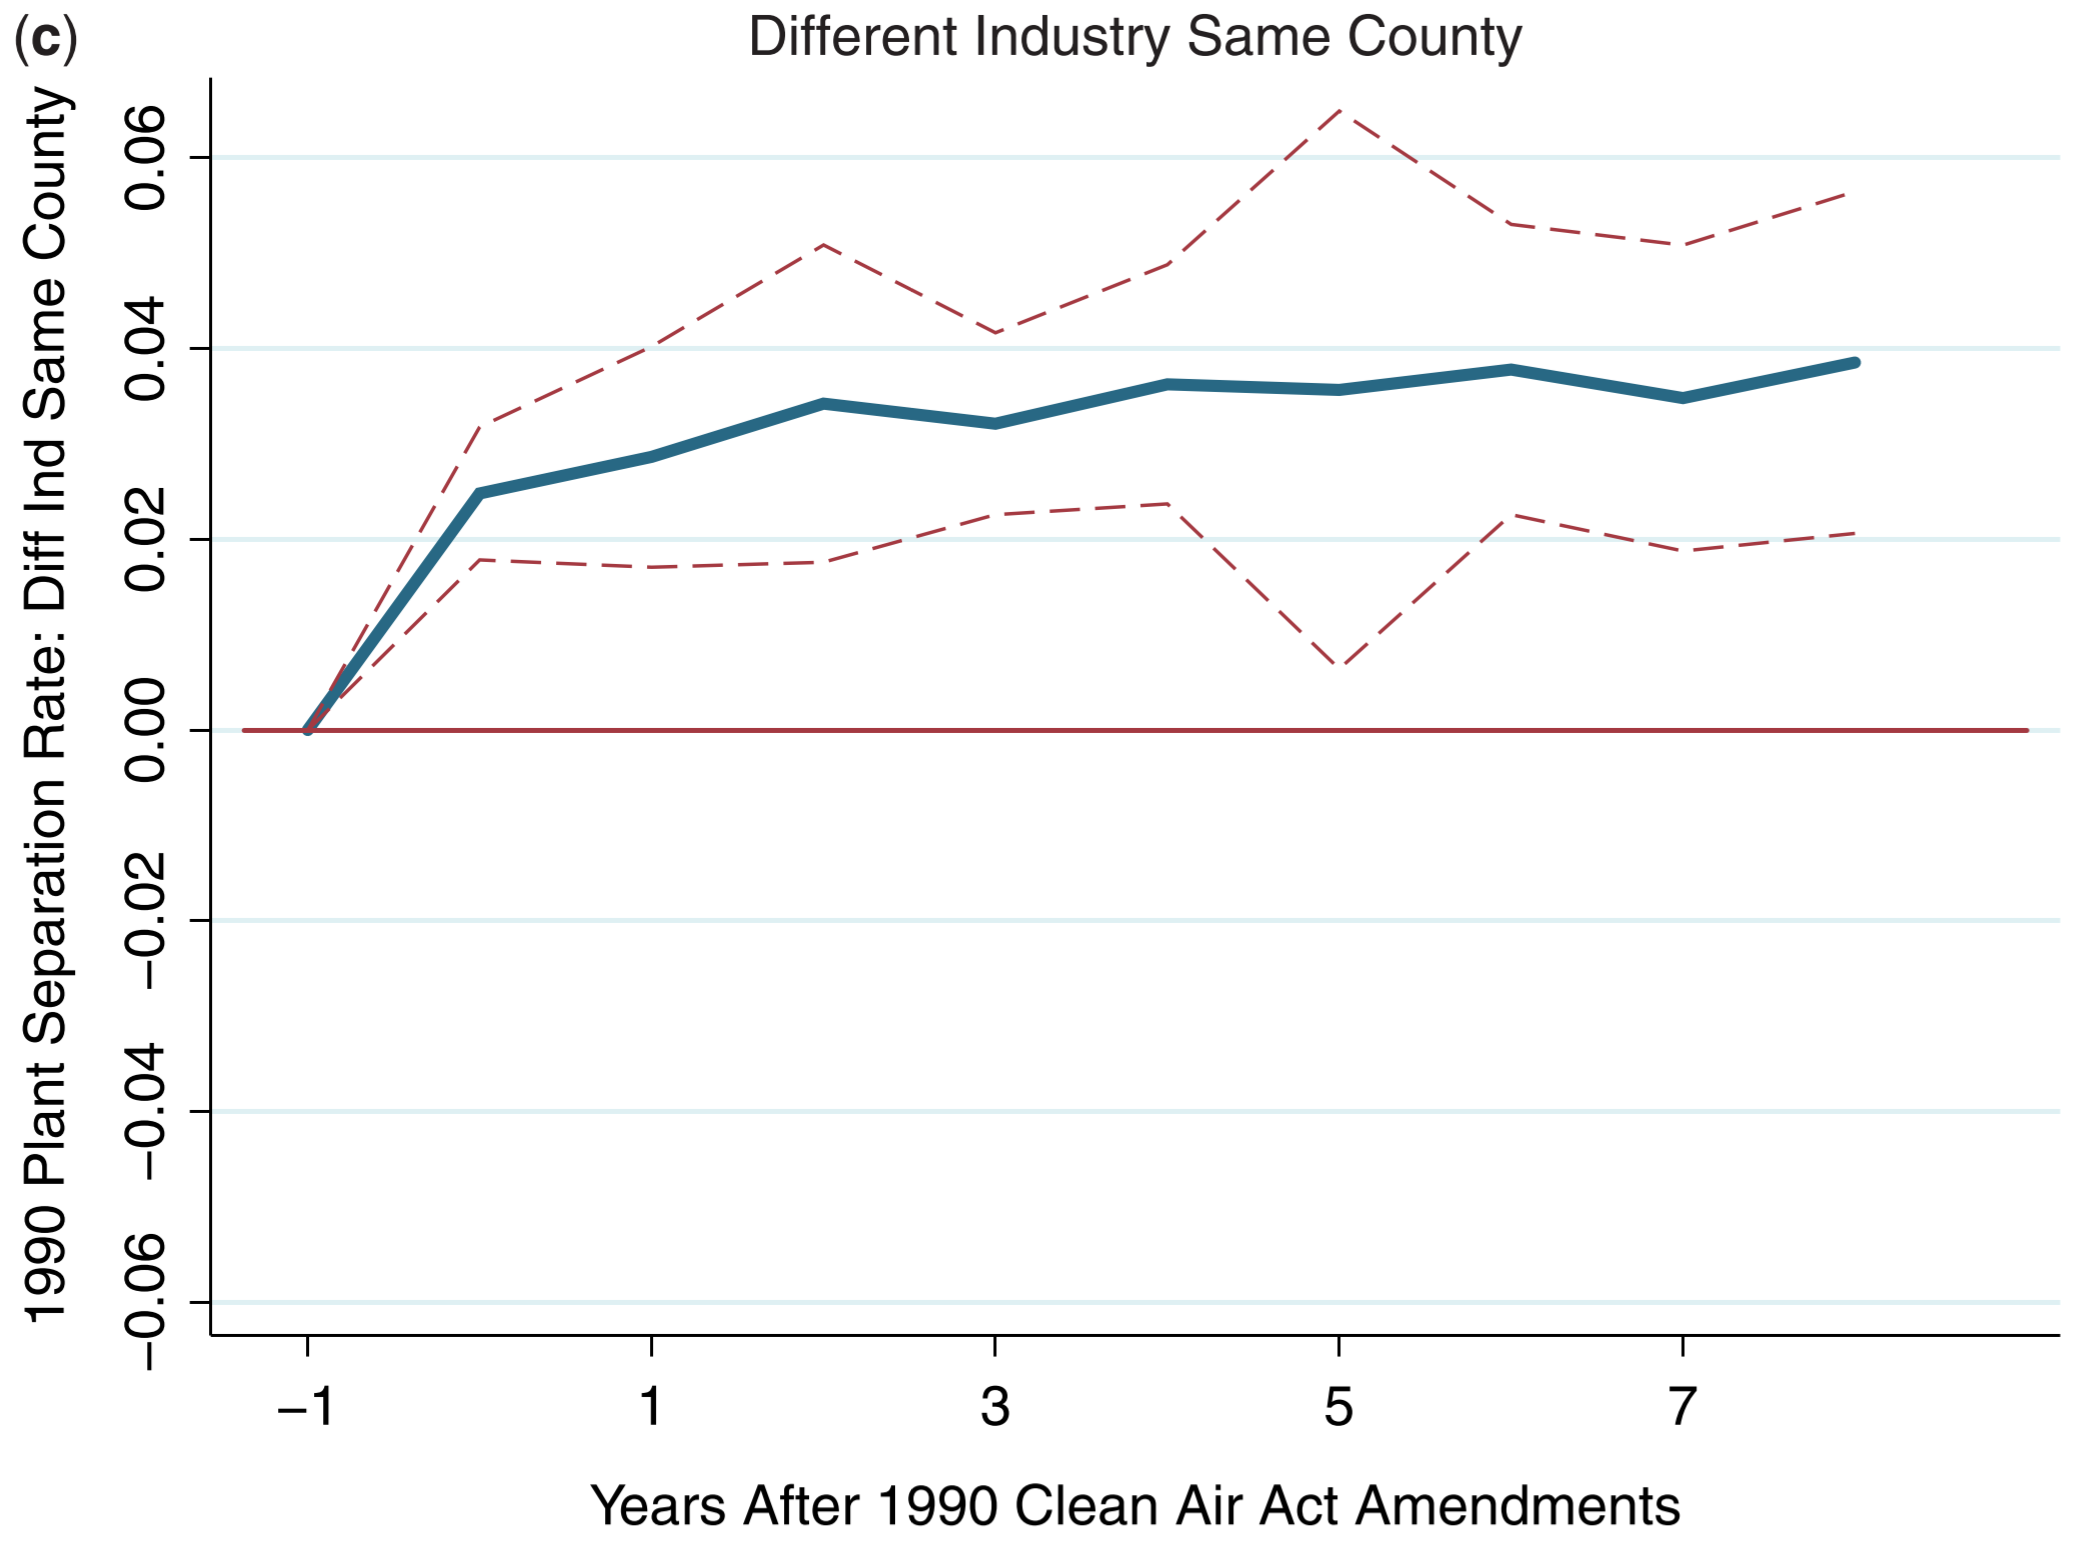
\includegraphics[scale=0.35]{figure6c.png}
	\end{figure}
\end{frame}
%------------------------------------------------
\begin{frame}{E. Mechanisms: Regulation Increases the Separation Rate and Time between Jobs}
	\begin{figure}[h]
		\centering
		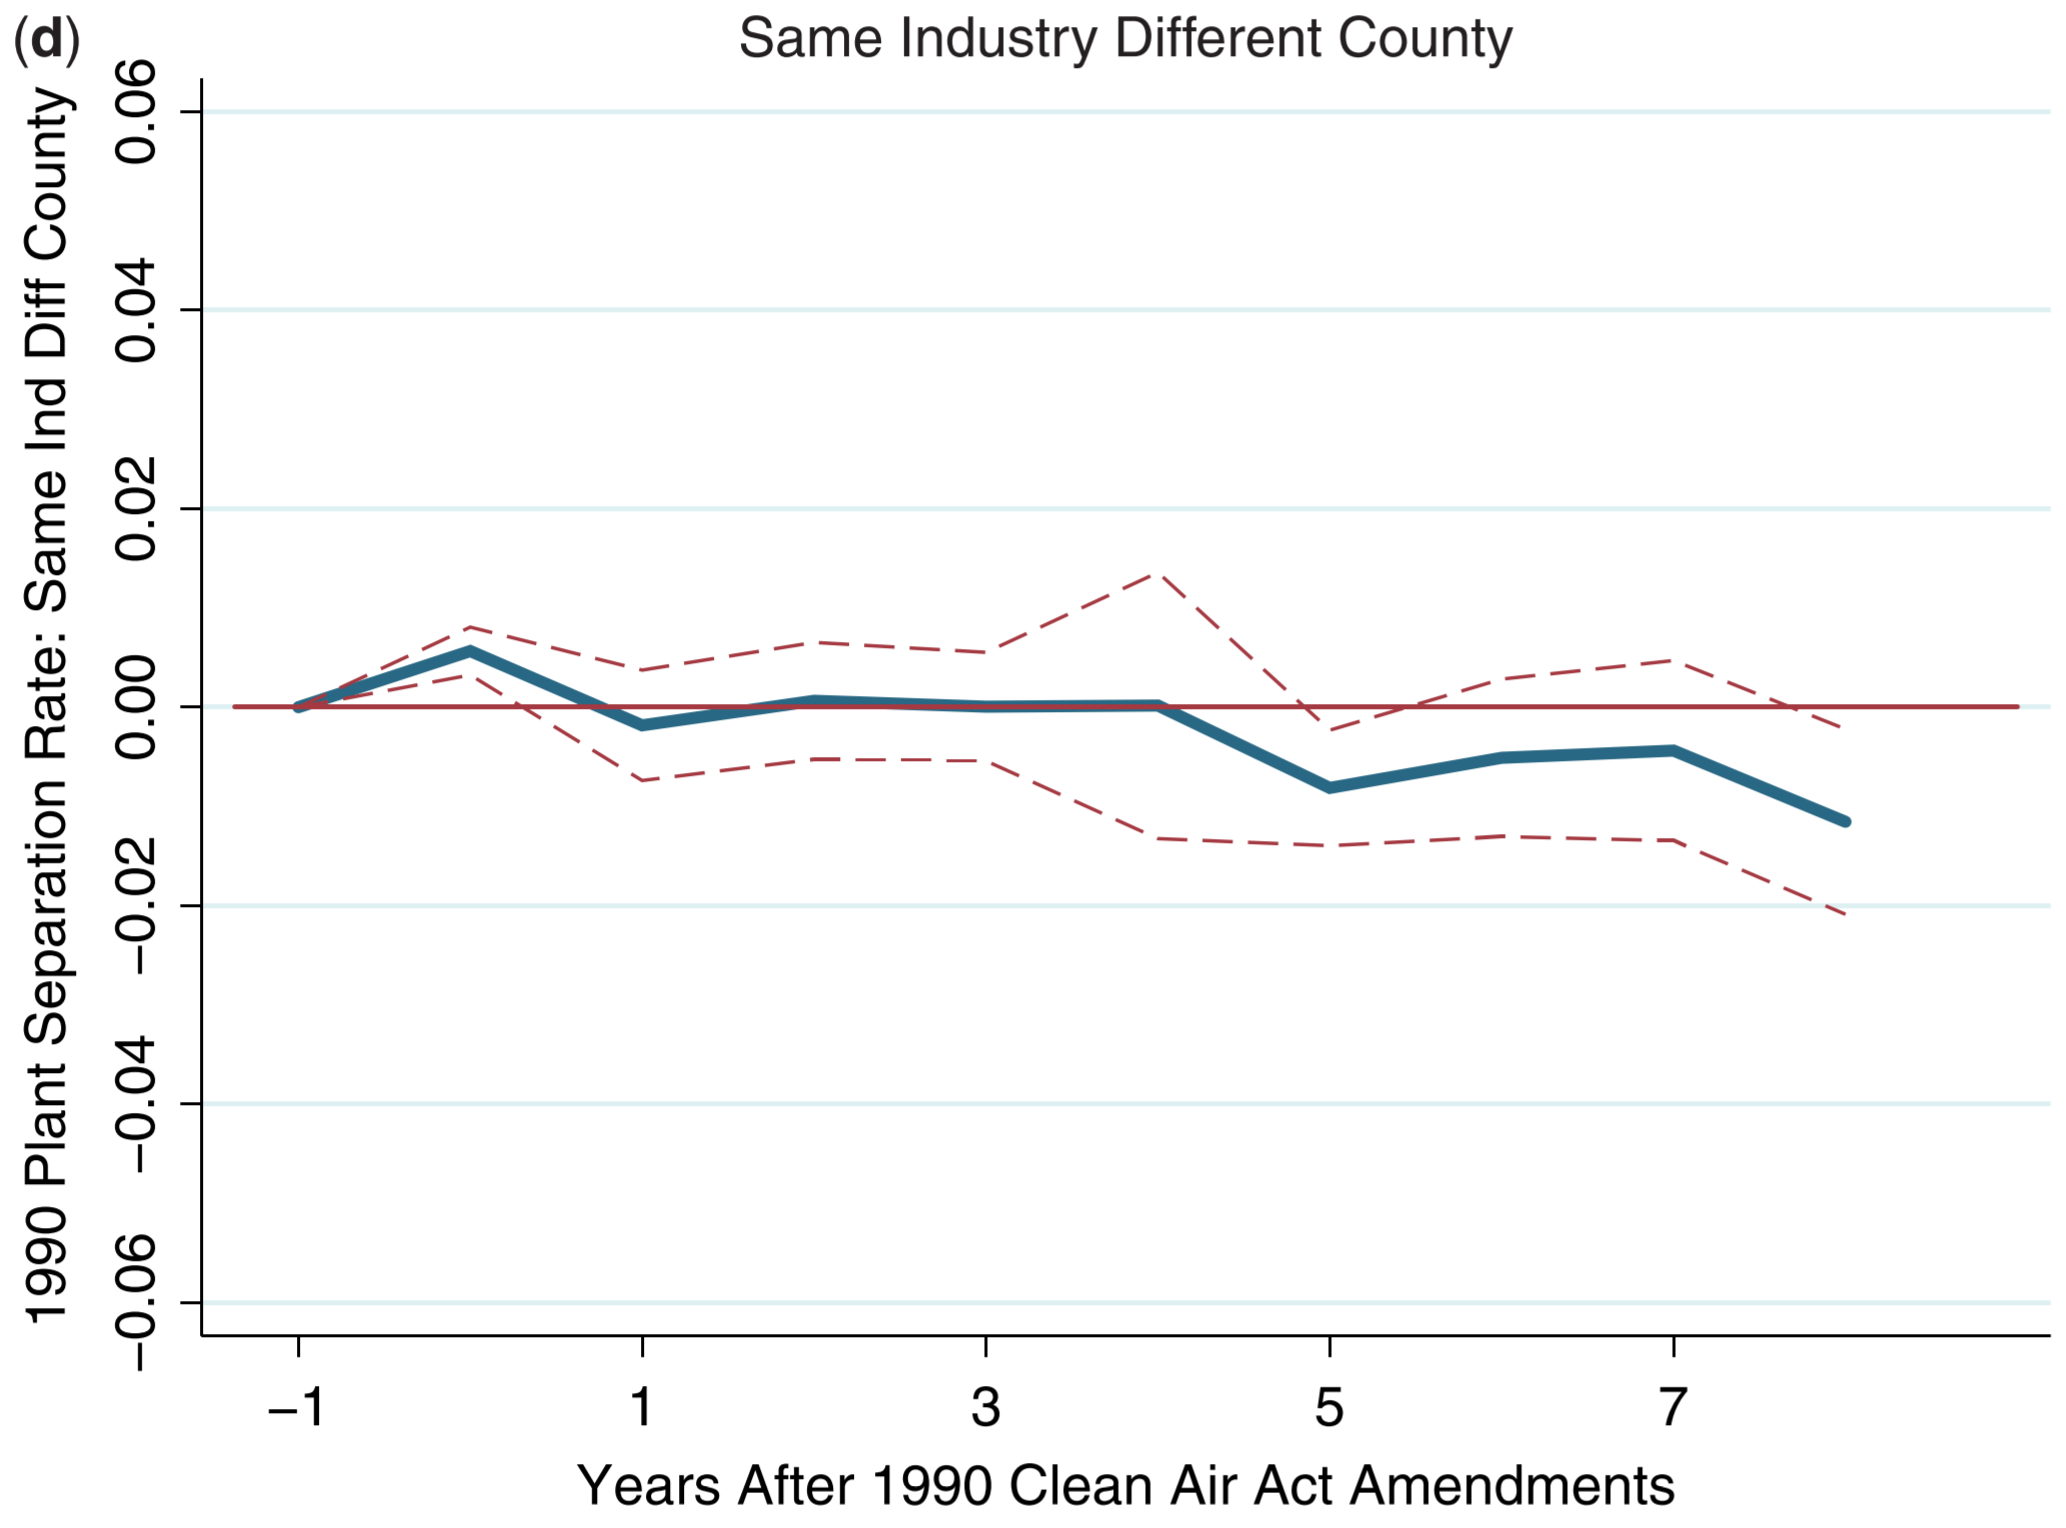
\includegraphics[scale=0.35]{figure6d.png}
	\end{figure}
\end{frame}
%-------------------------------------------------------------------------
%-------------------------------------------------------------------------
\section{Conclusion}
\begin{frame}[shrink]
	\transfade %fade in and fade out
	\tableofcontents[sectionstyle=show/shaded,subsectionstyle=show/shaded/hide]
	\addtocounter{framenumber}{-1}
\end{frame}
%------------------------------------------------
\begin{frame}{Conclusion}
	\textbf{Three primary contributions}
	\begin{enumerate}
		\item The reallocative costs of environmental policy in the context of worker outcomes is significant.
		\item The estimates shed light on how both firms and workers respond to gradual changes in regulatory stringency.
		\item Help understand the costs and consequences of labor market shocks in an economy where labor is not instantly reallocated and average industry wages may not fully reflect shifts in the labor demand curve.
	\end{enumerate}
	\textbf{Caveats}
	\begin{enumerate}
		\item Additional costs not captured by earnings alone;
		\item Many other labor market implications of environmental regulations not mentioned yet;
		\item Only partial equilibrium framework, cannot make precise inferences as to the overall economic effect or the economy more generally.
	\end{enumerate}
	\textcolor{red}{\textbf{Key point:} Regulations have distributional consequences.}
\end{frame}
%------------------------------------------------

%------------------------------------------------
\begin{frame}
\Huge{\centerline{\textit{The End}}}
\end{frame}
%-------------------------------------------------------------------------


\end{document} 